% Setup
\documentclass[a4 paper, 12pt]{article}

% Title
\title{COSC3000 - COMPUTER GRAPHICS REPORT \\ --- \\Olympics Athletic Track}
\author{Tean-louise Cunningham (42637460)}
\date{\today}

% Margins
\usepackage{geometry}
\geometry{margin=2cm}

% Images
\usepackage{graphicx}
\usepackage{float}
\usepackage[export]{adjustbox}
\setlength{\intextsep}{5pt plus 2pt minus 2pt}
\usepackage[font=small,skip=5pt]{caption}


% Paragraph
\setlength{\parindent}{2em}
\setlength{\parskip}{1em}

% Text Formatting
\usepackage[utf8]{inputenc}
\usepackage[english]{babel}

% List spacing
\usepackage{enumitem}
\setlist{noitemsep, topsep=0pt}
\setlist[enumerate]{parsep=5pt} 

% Text Color
\usepackage{xcolor}

% Hyperlinks
\usepackage{hyperref}
\hypersetup{
    colorlinks=true,
    linkcolor=black,
    filecolor=black,      
    urlcolor=blue,
}

% Appendix
\usepackage{appendix}

% Include pdf
\usepackage{standalone}
\usepackage{pdfpages}

% Borders
\usepackage{mdframed}

% Appendix
\usepackage{appendix}

\usepackage{listings}


%%%%%%%%%%%%%%%%%%%%%%%%%%%%%%%%%%%%%%%%%%
% DOCUMENT
\begin{document}

% Title
\maketitle
    \begin{figure} [H]
        \centering
        \includegraphics[width=0.95\textwidth]
            {./images/title.png}                  
    \end{figure}  


% Table of contents
\pagebreak
\tableofcontents
\pagebreak
\listoffigures

% INTRODUCTION
\pagebreak
\section{Introduction}
In continuance of the exploration of the Olympics from the visualisation project, a graphic simulation of running on an athletic track will be simulated. The main stadium of an Olympics is the most integral location as it hosts the opening and closing ceremonies, the lighting of the touch and the most popular events. The architecture and design choices of these stadiums ensure athletes can compete in optimal circumstances and thousands of spectators can experience these feats. This project will highlight the ingenuity of these stadiums by offering the opportunity to view its design in detail as a competitor on its athletic track. This will be achieved using the provided mega\_racer files, demo and instructions as a base, and the Tokyo National Stadium, which is set to host the 2020 Olympics as inspiration.

% MEGA RACER
\section{Mega Racer - Tier 1}

%% 1.1
\subsection{1.1 - Scale the terrain grid}
In terrain.py load() change zPos from 0 to the below to set the height of the terrain. Also, the last line from racer.py was uncommented so the racer can follow the height.   
    \begin{lstlisting}[language=python]
# terrain.py
def load(...):
    ...
    zPos = red * self.heightScale
    \end{lstlisting}

The height of the terrain is indicated by the shading of red in the provided track image and heightScale refers to appropriate height to x and y measurements given. 
    \begin{figure} [H]
        \centering
        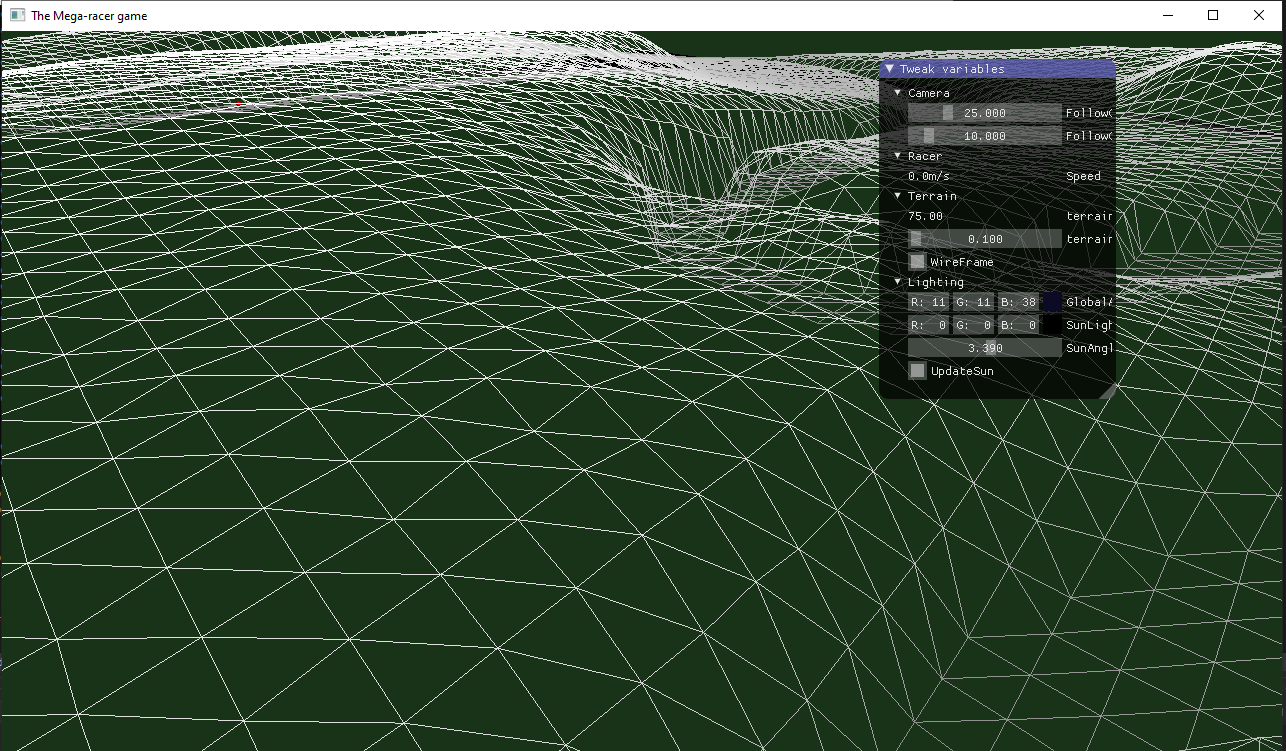
\includegraphics[width=0.8\textwidth, frame]
            {./images/mega_racer/1.1.PNG}
        \caption{1.1}
    \end{figure}  
   

%% 1.2
\subsection{1.2 - Set up a camera to follow the racer}
To start I looked at the code to understand what was happening and what each of the variables related to, particularly g\_viewPosition, g\_viewTarget and g\_viewUp. I found they were being called in mega\_racer.py in \textit{renderFrame()}:
    \begin{lstlisting}[language=python]
# mega_racer.py 
def renderFrame(...):
    ...
    view.worldToViewTransform = lu.make_lookAt(g_viewPosition, 
                                                g_viewTarget, 
                                                g_viewUp)
    \end{lstlisting}

Then I headed to \textit{make\_lookAt()} to see the functionality of the function and parameters that the arguments were being used for. The function makes a transformation from world to view space inversely by calling another function \textit{make\_lookFrom()} with a modified target parameter for smooth movement.  
    \begin{lstlisting}[language=python]
# lab_utils.py
def make_lookAt(eye, target, up):
    return make_lookFrom(eye, 
                        np.array(target[:3]) - np.array(eye[:3]), 
                        up)
    --> 
def make_lookFrom(eye, direction, up):
    .....
    \end{lstlisting}

Also, the examples from lab2 use similar functions in the same manner:
    \begin{lstlisting}[language=python]
# Lab 2 (1) - Q5
worldToViewTransform = magic.make_lookAt(eyePos, [0,0,0], [0,1,0])
# Lab 2 (2) 
worldToViewTransform = magic.make_lookFrom(g_cameraPosition,   
                                            cameraDirection, 
                                            [0,1,0])
    \end{lstlisting}
    
Therefore, the variables have the following meanings:
    \begin{itemize}
        \item g\_viewPosition = eye (location of camera, camera position)
        \item g\_viewTarget = target (point to aim, camera direction=target-eye)
        \item g\_viewUp = up (rough up direction)
    \end{itemize}    
    
With this understanding I could start to assign these variables appropriately to get the camera in the correct position. Firstly, it was clear that the 'target' needed to be updated to the position of the racer as this where the camera needs to be pointing. 
    \begin{lstlisting}[language=python]
# mega_racer.py
def update(...):
    ...
    g_viewTarget = g_racer.position
    \end{lstlisting}

Secondly, the position of the camera needed to be updated to take into account corresponding position of the racer for all coordinates. According to .... the 'desiredPosition = target.position + offset'. Thirdly, all coordinates of the of the camera needed to include the follow offset to be behind and above the racer. Additionally, the z coordinates needed to take into account the look offset of the camera as this is how it is looking at it from above.
    \begin{lstlisting}[language=python]
# mega_racer.py
def update(...):
    ...
    for i in range(0,3):
        g_viewPosition[i] = g_racer.position[i] 
                            + g_followCamOffset
    g_viewPosition[2] += g_followCamLookOffset
    \end{lstlisting}

After running these changes I could see that the camera was almost right, however it wasn't facing the correct direction; directly behind the racer. 
    \begin{figure} [H]
        \centering
        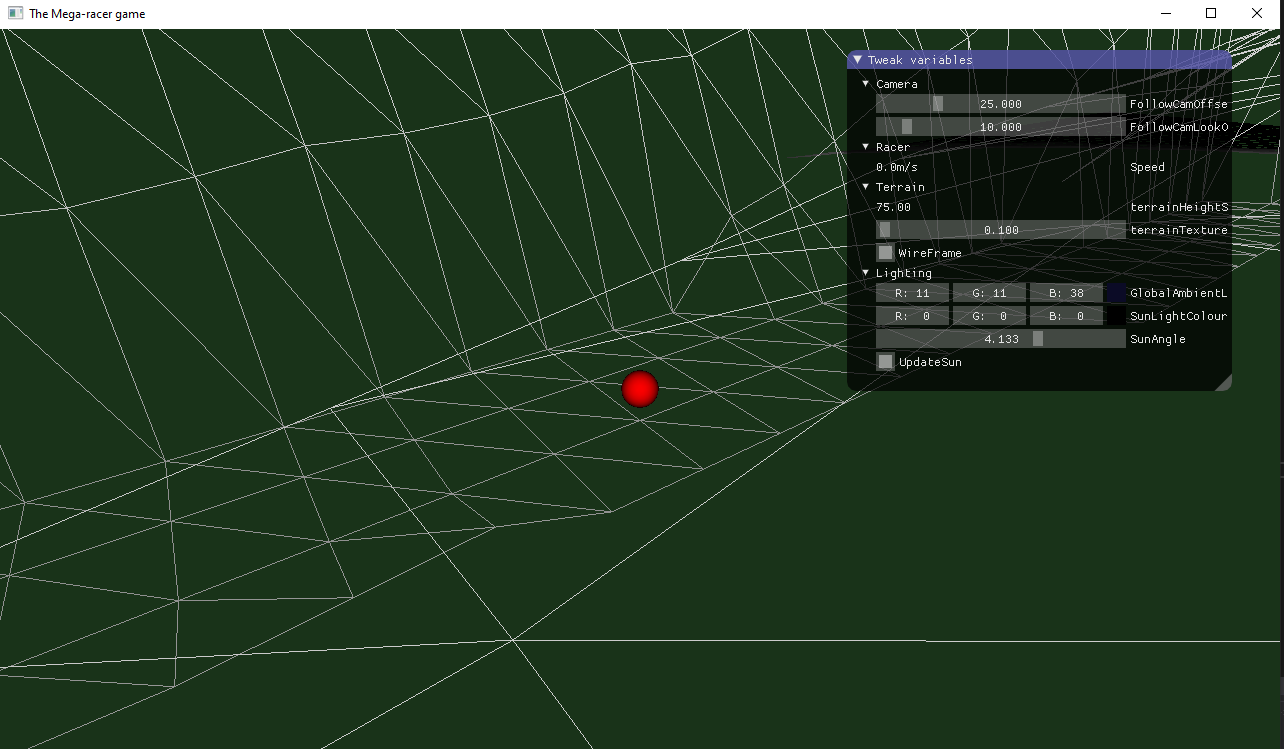
\includegraphics[width=0.8\textwidth, frame]
            {./images/mega_racer/1.2_a.PNG}
        \caption{1.2 - First Attempt}
    \end{figure}

On closer inspection of the Racer class I identified a variable called heading which controlled the direction of the racer. Since the camera needed to be behind the racer, the view position had to be multiplied by the inverse of the racer direction.
    \begin{lstlisting}[language=python]
# mega_racer.py
def update(...):
    ...        
    for i in range(0,3):
        g_viewPosition[i] = g_racer.position[i] 
                            + g_followCamOffset 
                            * -g_racer.heading[i]
    g_viewPosition[2] += g_followCamLookOffset
    \end{lstlisting}

This produced the correct result! The camera was now the position of the racer with the offsets applied at the appropriate direction to the racer's movement.
    \begin{figure} [H]
        \centering
        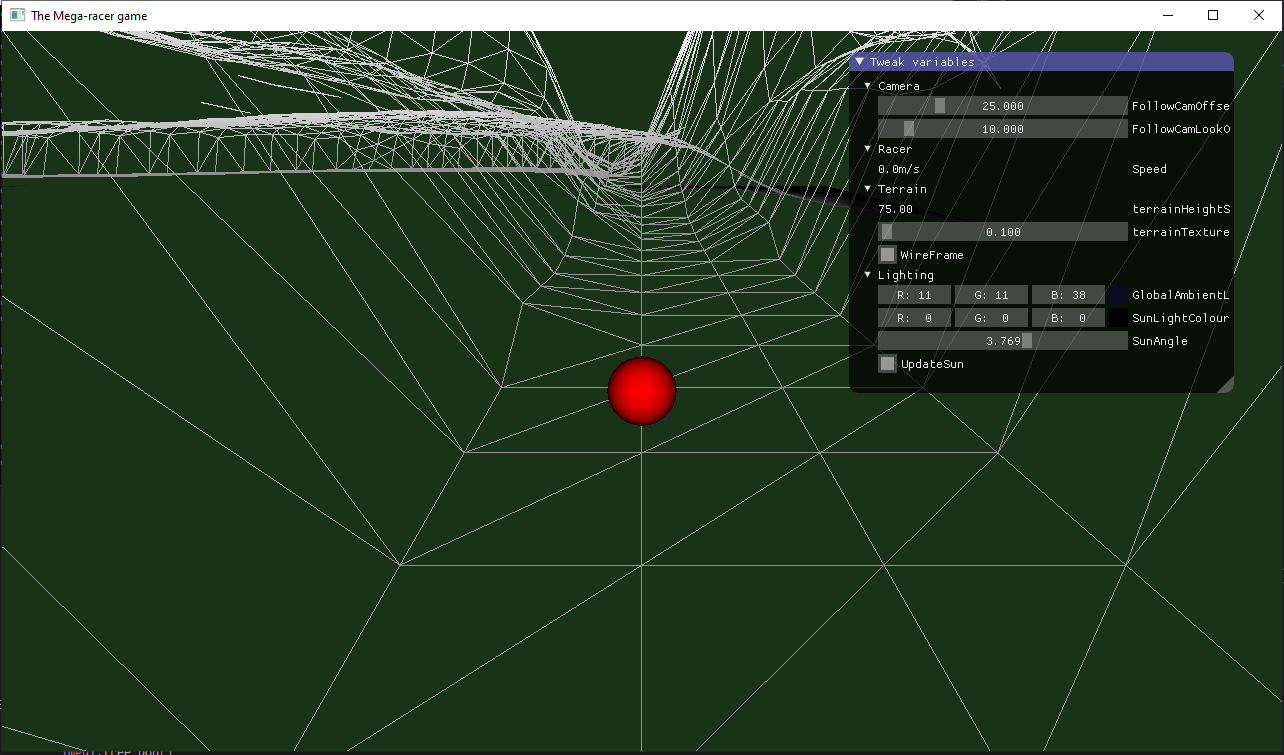
\includegraphics[width=0.8\textwidth, frame]
            {./images/mega_racer/1.2_b.PNG}
        \caption{1.2 - Final Attempt}
    \end{figure}  

%% 1.3
\subsection{1.3 - Place and orient a model for the racer}
Looking at the comments in the code I found two places with TODO for this section in racer.py; render() and load(). Starting with rendering the model I look at mega\_racer.py to see how this function was being called. The racer was being rendered in renderFrame().
    \begin{lstlisting}[language=python]    
# mega_racer.py
def renderFrame(...):
    ...
    g_racer.render(view, g_renderingSystem)  
-->
#racer.py - Racer
def render(self, view, renderingSystem):
    .....
    \end{lstlisting}  

The the view is of ViewParams class and is set up to project and transform from view to clip space, and world to view space. The renderingSystem parameter is of RenderingSystem class. The task for render() is to draw the model and this class has the drawObjModel() function mentioned in the project notes that needs to be used. This function call is added to Racer.render(). In the Racer class there is model variable set to None, and view is passed in as an argument to render(). The only missing parameter is the modelToWorldTransform.
    \begin{lstlisting}[language=python]   
# mega_racer.py - RenderingSystem
def drawObjModel(self, model, modelToWorldTransform, view):
    ...
        -->
# racer.py - Racer
def render(self, view, renderingSystem):
    renderingSystem.drawObjModel(self.model, ???, view)
    \end{lstlisting}  

The project notes mention make\_mat4\_from\_zAxis() as a useful function for transforming the model to the world. This function is in the lab\_utils file (imported as lu in racer.py). The function takes the parameters translation, zAxis and yAxis. The zAxis represents forwards and the yAxis represents up. Therefore, for this world, the z an y axis will act conventionally to the same. This means that the z-axis is the same as the direction of the racer (the heading) and the y-axis is equal to up view of the racer as determined by g\_viewUp in mega\_racer.py. The translation parameter refers to the position of model after all the relevant modifications to the coordinates, in this case that is the position of the racer.
    \begin{lstlisting}[language=python]  
#lab_utils.py    
def make_mat4_from_zAxis(translation, zAxis, yAxis):
    ...
-->
# racer.py - Racer
def render(...):
    modelToWorldTransform = lu.make_mat4_from_zAxis(self.position, 
                                                    self.heading, 
                                                    [ 0.0, 0.0, 1.0 ])
    \end{lstlisting}

After running this code, there was an error message relating to the model; it is of none type. So the next step is to create and load the racer model in load(). 
    \begin{figure} [H]
        \centering
        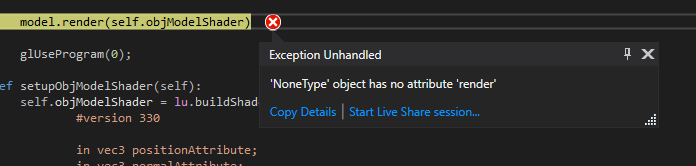
\includegraphics[width=0.8\textwidth, frame]
            {./images/mega_racer/1.3_a.PNG}
        \caption{1.3 -Error}
    \end{figure}

Looking at mega\_racer.py the load() method is called with three parameters; the object file for the racer, the terrain and the rendering system. The purpose of the load() function is to create and load the model. 
    \begin{lstlisting}[language=python]
# mega_racer.py
g_racer.load("data/racer_02.obj", g_terrain, g_renderingSystem)
-->
# racer.py - Racer
def load(self, objModelName, terrain, renderingSystem):
        .....    
    \end{lstlisting}

The rendering system there seemed to be no relevant functions. In the project notes there was mention that the Racer class relied on the ObjModel class, and since drawObjModel() draws ObjModel's then the racer model needed to be an instance of this class. Looking at ObjModel\_\_init\_\_() the only requirement argument is the filename which is given.
    \begin{lstlisting}[language=python]
    self.model = ObjModel(objModelName)
    \end{lstlisting}   

Now the model for the racer has replaced the red dot and the movement relating to the arrows in accurate.
\begin{figure} [H]
    \centering
    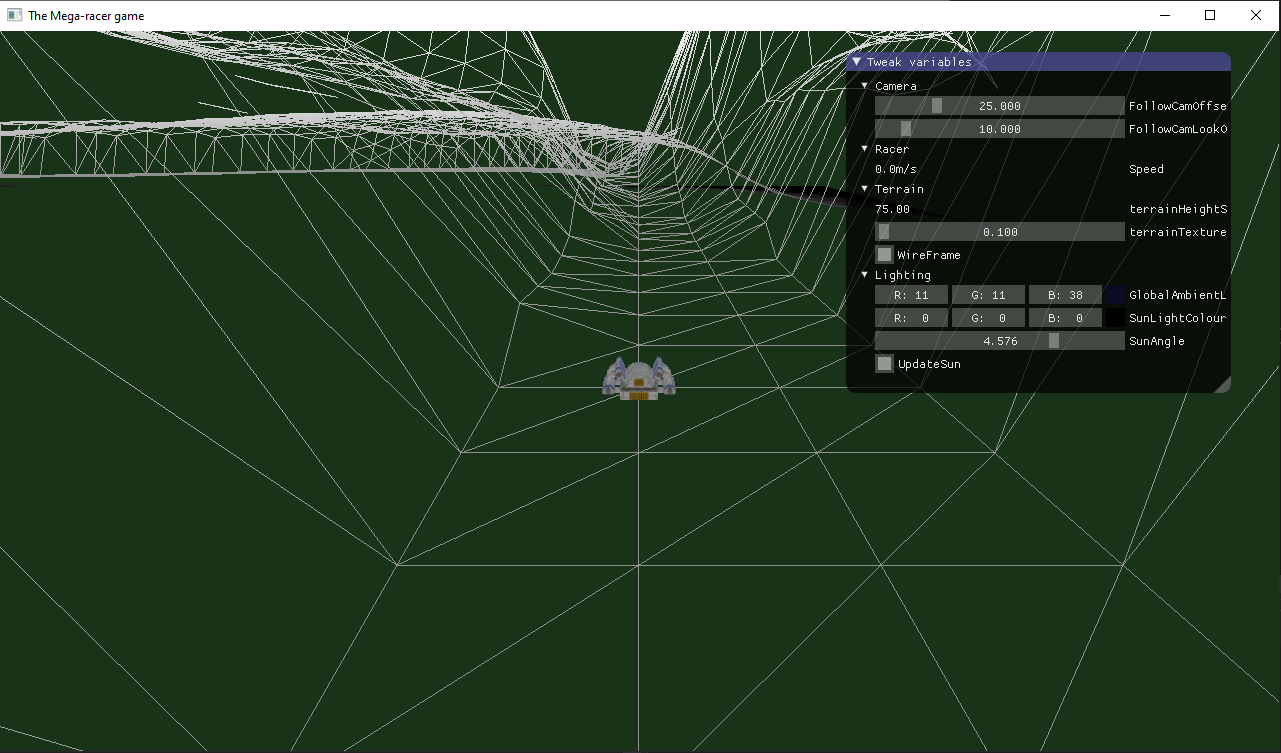
\includegraphics[width=0.8\textwidth, frame]
        {./images/mega_racer/1.3_b.PNG}
    \caption{1.3 - Final}
\end{figure}

%% 1.4
\subsection{1.4 - Texture the terrain}
There are three steps to complete this section in terrain.py. 

\textbf{(1) render() - need to bind the grass texture to the right texture unit.} \\ 
The hint is to is to use lu.bindTexture. This function, bindTexture(), takes two arguments texUnit and textureId. A similar function is used in lab\_utils.py (Lab Code, 2020), also called bindTexture(). In order to use the bindTexture in render() for the project I looked at how it was called in lab 5 question 12 (Lab Code, 2020).
    
    \begin{lstlisting}[language=python]
# Lab - lab_utils.py 
def bindTexture(texUnit, textureId, textureType = GL_TEXTURE_2D):
    ...
    -->
# Lab 5 Q12 - lab_5_template_2.py
g_detailTexture = None
def renderFrame(...):
    .....
    lu.bindTexture(0, g_detailTexture)
    lu.setUniform(g_shaderProgram, "baseTexture", 0)
    \end{lstlisting}

The textureId was first declared and then passed in and the texUnit set to 0. In terrain.py the texUnit is given as TU\_Grass (also equal to 0) and the textureID needs to be declared. Additionally, setUniform() needs to be called to set the shader. Updating the variable names the same was added to terrain.py.
    \begin{lstlisting}[language=python]       
# terrain.py
grassTexture = None

def render(...):
    ....
    lu.bindTexture(self.TU_Grass, self.grassTexture)
    lu.setUniform(self.shader, "grassTexture", self.TU_Grass)        
    \end{lstlisting}

   
\textbf{(2) load(): Compute the texture coordinates and sample the texture for the grass and use as material colour.} \\
As per the project notes the variable textureXyScale is to be used to scale the texture coordinates and is already set to a factor of 0.1 so the texture repeats every 10 metres. Also the world space coordinates should be used  to sample the texture in the fragment shader. To determine how to set the sample I looked at Lab 5 question 12 which sets the colours of the texture in the fragment shader.
\begin{lstlisting}[language=python] 
# Lab 5 - Q12   
def initResources():
    .....         
    in vec2 v2f_textureCoord;
    uniform sampler2D detailTexture; 
    uniform float texCoordScale; 
    out vec4 fragmentColor;
    void main() 
    {...
        vec3 detailColour = texture(detailTexture, 
                            v2f_textureCoord * texCoordScale).xyz;      
        fragmentColor = vec4(detailColour, 1.0);
    }        
\end{lstlisting}

From this example it is evident that the three arguments for texture() need to be assigned to the new materialColour (i.e. detailColour).
    \begin{itemize}
        \item detailTexture: The grass colour is similar to the detailColour so the detailTexture is equivalent to the grassTexture.
        \item texCoordScale: In lab 5 the v2f\_textureCoord is a 2 dimensional out vector from the vertex shader. As per the project notes, since the vertex is regular, we can replicate this same behaviour by only selecting the x and y coordinates of the world space which are stored in v2f\_worldSpacePosition.
        \item v2f\_textureCoord: The textCoordScale in lab 5 is a new name for the given g\_texCoordScale which is declared and uniformly set for the shader as texCoordScale. The same is done for textureXyScale in Terrain which as mentioned is nominated in the project notes as the scale for the texture coordinates.
    \begin{lstlisting}[language=python] 
# Lab 5 
g_texCoordScale = 7.0
def renderFrame():
    .....
    lu.setUniform(g_shaderProgram, "texCoordScale", g_texCoordScale)

# terrain.py
textureXyScale = 0.1
def render():
    lu.setUniform(self.shader, 
                    "terrainTextureXyScale", 
                    self.textureXyScale);
    \end{lstlisting}
    \end{itemize}

Putting this all together we get the following code to calculate the coordinates and sample the texture for the grass, overriding the existing material colour.
    \begin{lstlisting}[language=python] 
# terrain.py - Terrain
def load(...):
    ...
    fragmentShader =
        ...
        void main()
        {
            vec3 grassColour = texture(grassTexture, 
                                        v2f_worldSpacePosition.xy 
                                            * terrainTextureXyScale).xyz;
            materialColour = grassColour;
            ...
        }
    \end{lstlisting}

\textbf{(3) load() - fragmentShader: Load texture and configure the sampler.} \\
Also in lab 5, in initResources() after declaring the shader the image is opened and the texture is mapped (glTextParameter), then the texture is loaded using lu.loadTexture(). A similar function can be found in the ObjModel.py (instead of lab\_utils.py) and performs the same actions. It also sets the texture to wrap repeatedly as desired.
    \begin{lstlisting}[language=python]   
# Lab 5 
g_detailTexture = lu.loadTexture("data/details.jpg");
--> 
def loadTexture(fileName): 
    ....

# ObjModel.py - ObjModel
def loadTexture(self, fileName, basePath, srgb):
    ......
    glTexParameteri(GL_TEXTURE_2D, GL_TEXTURE_WRAP_S, GL_REPEAT);
    glTexParameteri(GL_TEXTURE_2D, GL_TEXTURE_WRAP_T, GL_REPEAT);
    \end{lstlisting}

To load the texture for the terrain this function needs to be called with the relevant parameters.
    \begin{lstlisting}[language=python]   
# terrain.py - Terrain
def load(...):
    self.grassTexture = ObjModel.loadTexture("grass2.png", "data", True)
    \end{lstlisting}

\begin{figure} [H]
    \centering
    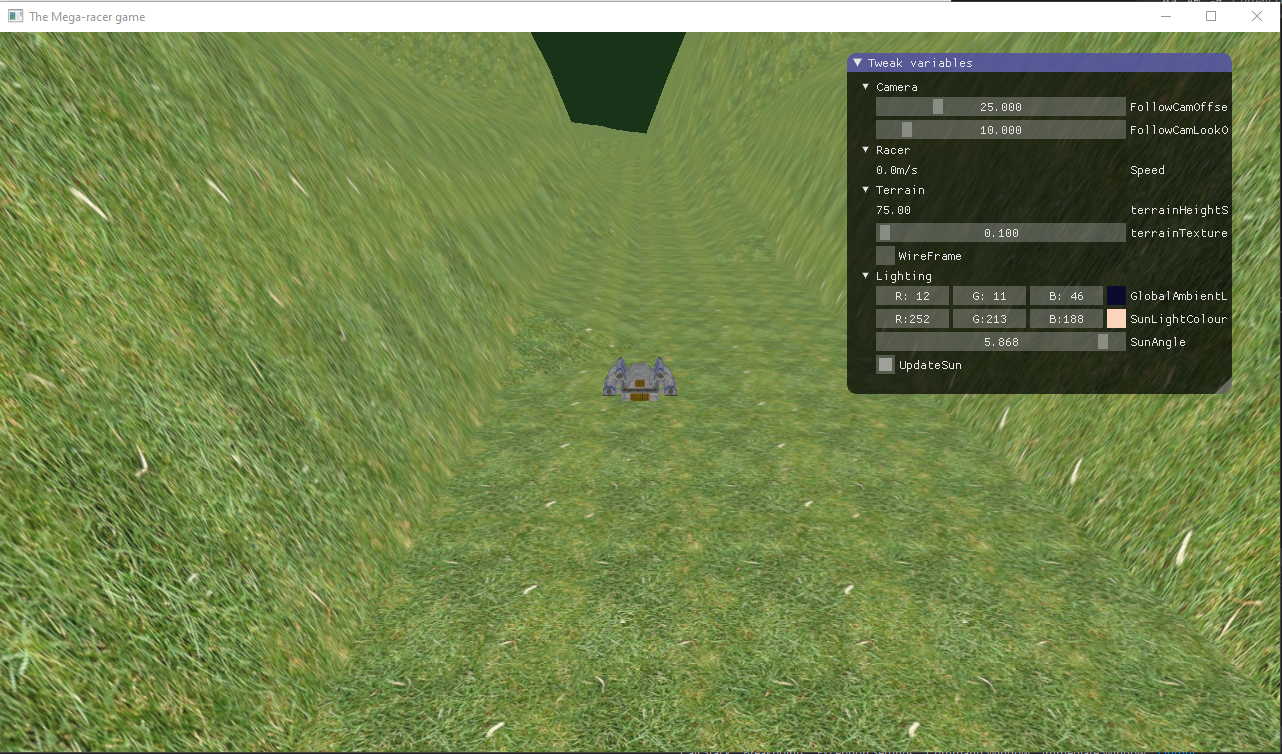
\includegraphics[width=0.8\textwidth, frame]
        {./images/mega_racer/1.4.PNG}
    \caption{1.4 - Final}
\end{figure}



\subsection{1.5 Lighting from the sun}  

The project notes explain that the code for the light should be added to the computeShading() function in RenderingSystem class as part of the commonFragmentShaderCode variable. This function is called in setUpModelShader() where the viewSpaceNormal and viewSpacePosition variables are declared by the vertex shader, materialColour is declared as materialDiffuse in the fragment shader, and viewSpaceLightPosition and sunLightColour are carried over from the commonShaderCode variable. 
    \begin{lstlisting}[language=python] 
#  mega_racer.py - RenderingSystem
def setupObjModelShader(...):
    v2f_viewSpaceNormal = normalize(modelToViewNormalTransform * normalAttribute);
    v2f_viewSpacePosition = (modelToViewTransform * vec4(positionAttribute, 1.0)).xyz;
    .....
    vec3 materialDiffuse = texture(diffuse_texture, 
                                    v2f_texCoord).xyz 
                                    * material_diffuse_color;
    vec3 reflectedLight = computeShading(materialDiffuse, 
                                            v2f_viewSpacePosition, v2f_viewSpaceNormal, viewSpaceLightPosition, 
                                            sunLightColour
                                        ) + material_emissive_color;
    \end{lstlisting}

A couple of things to keep in mind:
    \begin{itemize}
        \item position of sun = g\_sunPosition: The sun is set to move around around the world.
        \item colour of sunlight = g\_sunLightColour = lightColour
        \item all parameters om shading must be the same space -> set as view space (same as lab 4) 
        \item sun is defined in world space
        \item The computeShading function needs to be called from each function -> this is already done.
        \item Need to make sure don't just have Lambertian term -> Fixed by multiplying by materialDiffuse term.
        \item Use clamping to check when light is behind surface
    \end{itemize}


To create the lighting effect required, all of the code followed that of fragmentShader.glsl in Lab 4. Question 1 was already provided as a basic shader. The view space is used for shading calculations. The computeShading() function is setup with five parameters, all of which are used to return a light value.
    \begin{lstlisting}[language=python] 
# mega_racer.py - RenderingSystem
commonFragmentShaderCode =
    ...
    vec3 computeShading(vec3 materialColour, 
                        vec3 viewSpacePosition, 
                        vec3 viewSpaceNormal, 
                        vec3 viewSpaceLightPos, 
                        vec3 lightColour)
    {
        return lightValue;
    }
    \end{lstlisting}

\textbf{(1) The direction towards the source of the light.} \\
Starting from Lab 4, question 2, the first step is to compute the normalised direction towards the light from the shading point in view space. The light position is stored as viewSpaceLightPosition and the current point is viewSpacePosition (provided by the vertex shader). 
    \begin{lstlisting}[language=python] 
# Lab 4 - Q2 - FragmentShader
vec3 viewSpaceDirToLight = normalize(viewSpaceLightPosition - viewSpacePosition);
    
# mega_racer.py - RenderingSystem
commonFragmentShaderCode =
    ...
    vec3 computeShading(...)
    {
        vec3 viewSpaceDirToLight = normalize(viewSpaceLightPos- viewSpacePosition);
        return viewSpaceDirToLight;
    }
    \end{lstlisting}

    \begin{figure} [H]
        \centering
        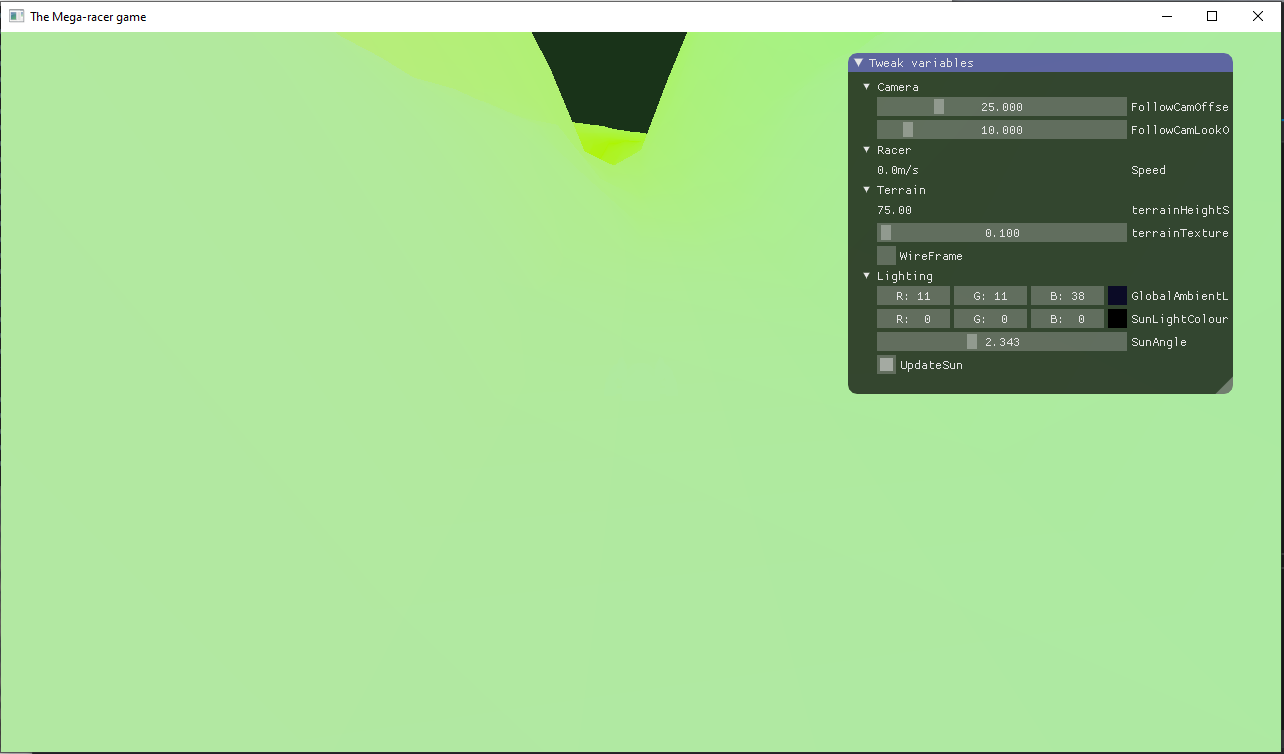
\includegraphics[width=0.8\textwidth, frame]
            {./images/mega_racer/1.5_a.PNG}
        \caption{1.5 - Step 1}
    \end{figure}

\textbf{(2) Compute the incoming light intensity.}
Use the calculated direction to calculate the incoming light intensity. As mentioned, in mega\_racer.py three variable of viewSpaceNormal is already provided by the vertex shader. This maintains the unit-length property of the normal.
    \begin{lstlisting}[language=python] 
# Lab 4 - Q2 - FragmentShader
vec3 viewSpaceNormal = normalize(v2f_viewSpaceNormal);
float incomingIntensity = max(0.0, dot(viewSpaceNormal, viewSpaceDirToLight));

# mega_racer.py - RenderingSystem
commonFragmentShaderCode =
    ...
    vec3 computeShading(...)
    {
        ...
        float incomingIntensity = max(0.0, dot(viewSpaceNormal, viewSpaceDirToLight));
        return incomingIntensity;
    }
    \end{lstlisting}

    \begin{figure} [H]
        \centering
        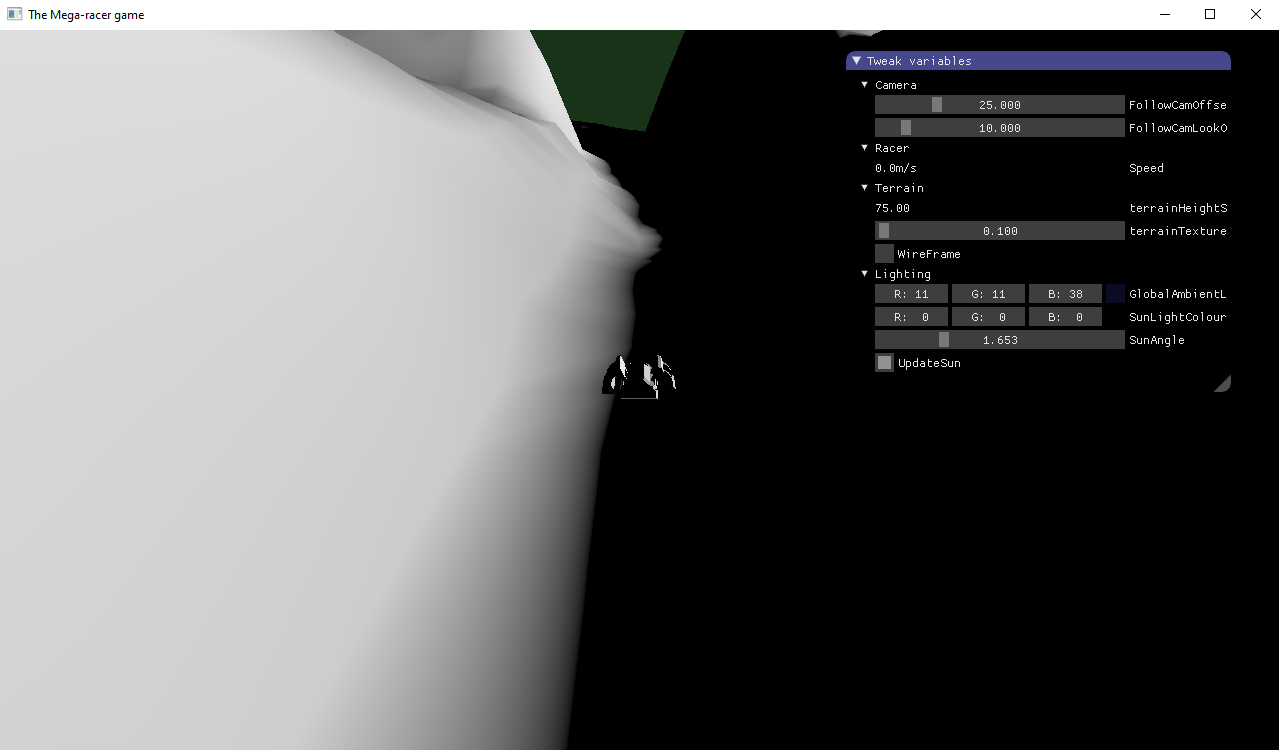
\includegraphics[width=0.8\textwidth, frame]
            {./images/mega_racer/1.5_b.PNG}
        \caption{1.5 - Step 2}
    \end{figure}


\textbf{(3) Modify the light that is emitted by the light source to have the correct colour and maximum intensity.}
This fixes the proportion if incoming light arriving at the surface so it is the correct colour and maximum intensity
    \begin{lstlisting}[language=python] 
# Lab 4 - Q2 - FragmentShader
vec3 incomingLight = incomingIntensity * lightColourAndIntensity;

# mega_racer.py - RenderingSystem
commonFragmentShaderCode =
    ...
    vec3 computeShading(...)
    {
        ...
        vec3 incomingLight = incomingIntensity * lightColour;
        return incomingLight;
    }        
    \end{lstlisting}

    \begin{figure} [H]
        \centering
        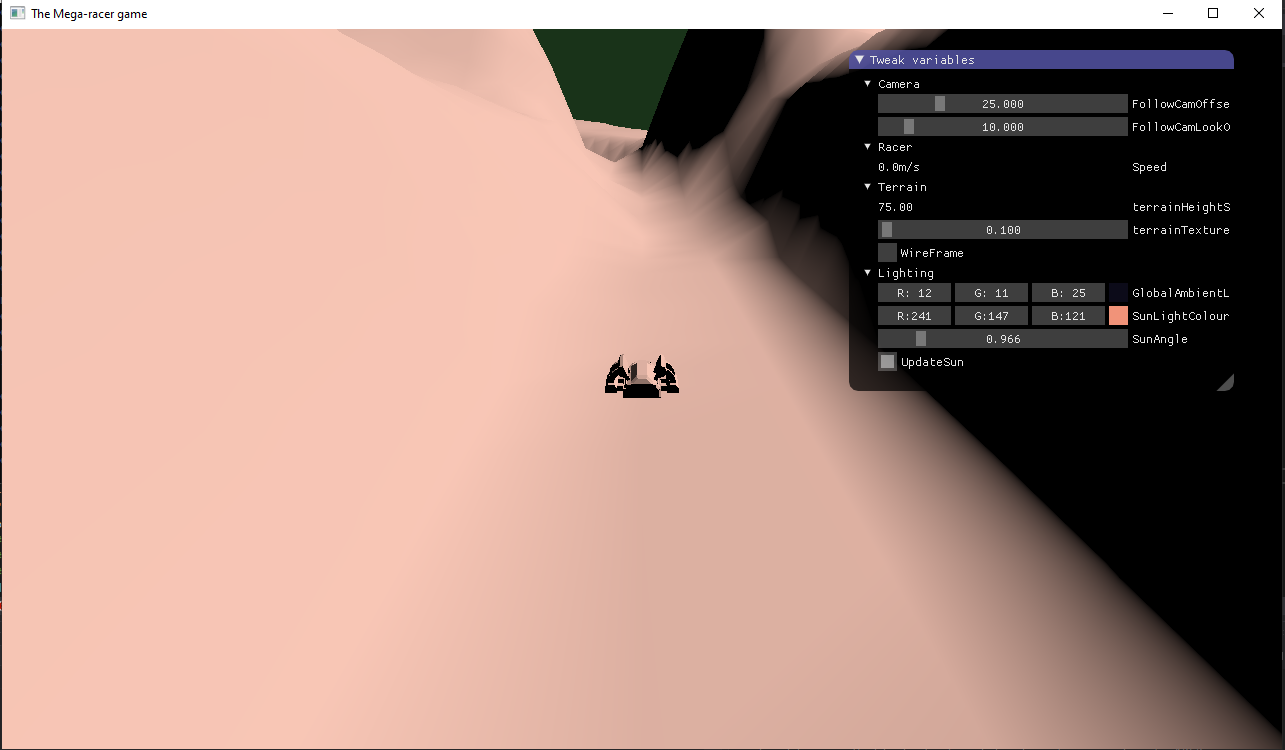
\includegraphics[width=0.8\textwidth, frame]
            {./images/mega_racer/1.5_c.PNG}
        \caption{1.5 - Step 3}
    \end{figure}


\textbf{(4) Diffuse Lambertian Reflection.}
Moving on to question 3 of lab 4, the next step is to diffuse the Lambertian reflection by multiplying the incoming light with a constant that represents the reflection of the material for the given spectrum. The argument passed as materialColour should provide this representation, as provided by the materialDiffuse variable passed in to computeShading() in setUpObModelShader(). This variable follows the same pattern as that of lab 4.  
    \begin{lstlisting}[language=python] 
# Lab 4  - FragmentShader
vec3 materialDiffuse = texture(diffuse_texture, v2f_texCoord).xyz * material_diffuse_color;
vec3 outgoingLight = incomingLight * materialDiffuse;

# mega_racer.py - RenderingSystem
commonFragmentShaderCode =
    ...
    vec3 computeShading(...)
    {
        ...
        vec3 outgoingLight = incomingLight * materialColour;
        return outgoingLight;
    }                            
    \end{lstlisting}

    \begin{figure} [H]
        \makebox[\textwidth]{%
        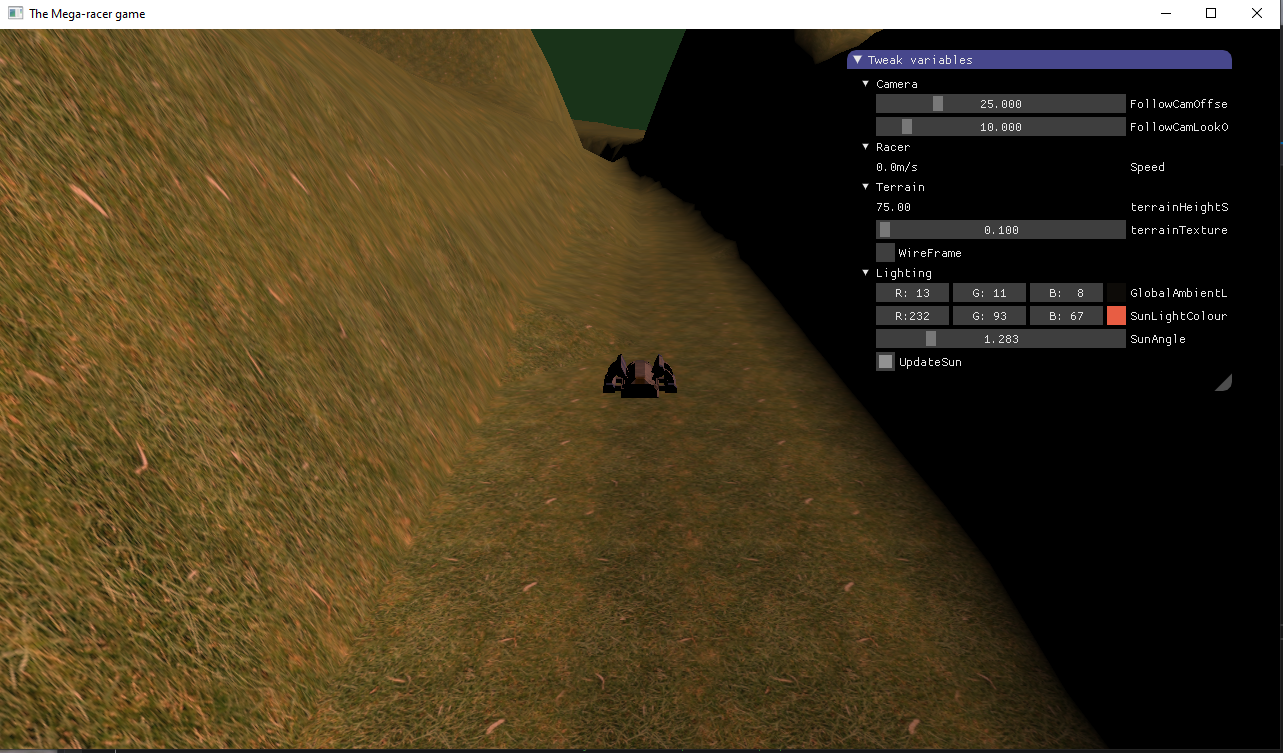
\includegraphics[width=0.49\textwidth, frame]
            {./images/mega_racer/1.5_d_1.PNG}%
        \hfill
        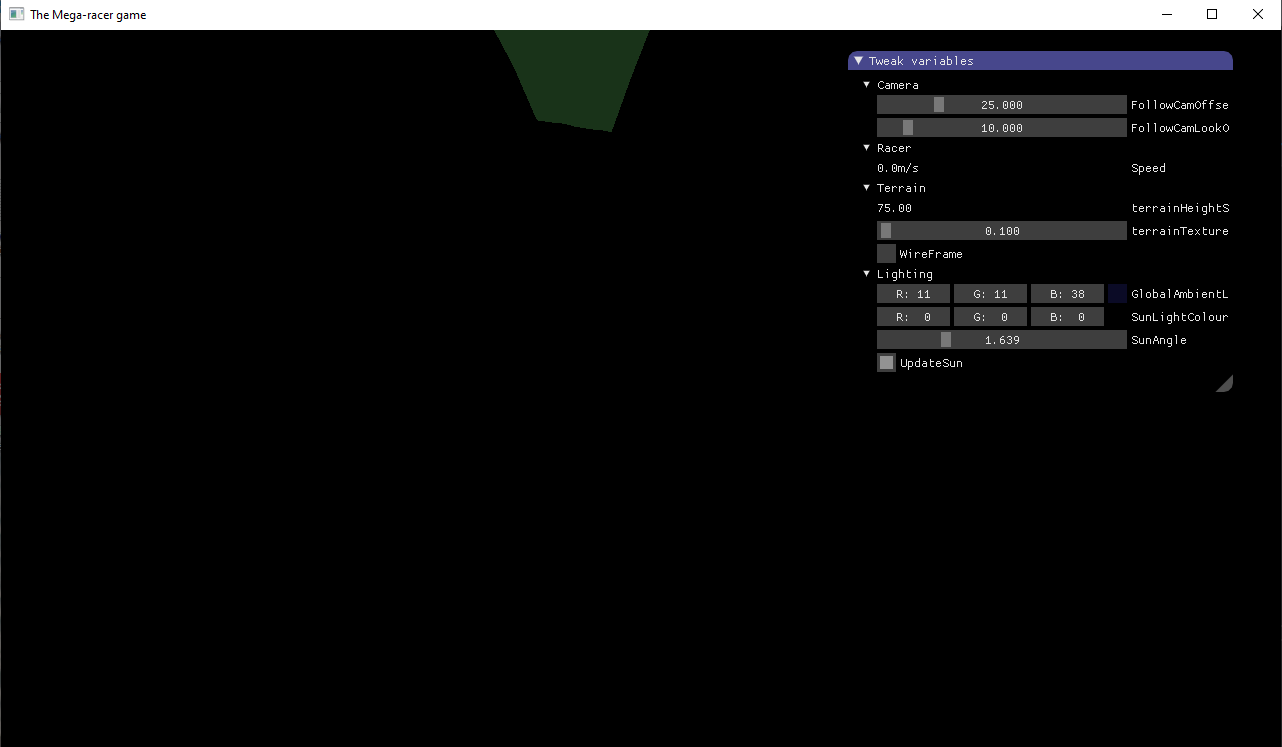
\includegraphics[width=0.49\textwidth, frame]
            {./images/mega_racer/1.5_d_2.PNG}
        }        
        \caption{1.5 - Step 5}   4
    \end{figure}

\textbf{(5) Take into account the indirect light.}
The next step is to handle the ambient light. This step builds on step 3 and follows question 4 in lab 4. As mentioned in the notes, this is an approximation with a single colour value. The ambience is added to the incomingLight variable as there is the light comes from everywhere, and then multiplied by the BRDF as both are independent.
    \begin{lstlisting}[language=c++] 
# Lab 4  - FragmentShader
vec3 outgoingLight = (incomingLight + ambientLightColourAndIntensity) 
                        * materialDiffuse;

# mega_racer.py - RenderingSystem
commonFragmentShaderCode =
    ...
    vec3 computeShading(...)
    {
        ...
        vec3 outgoingLight = (incomingLight + globalAmbientLight) 
                            * materialColour;
        return outgoingLight;
    }       
    \end{lstlisting}

This has produced the final results, light that doesn't cause pitch black and reflects according to the correct colour.
    \begin{figure} [H]
        \makebox[\textwidth]{%
        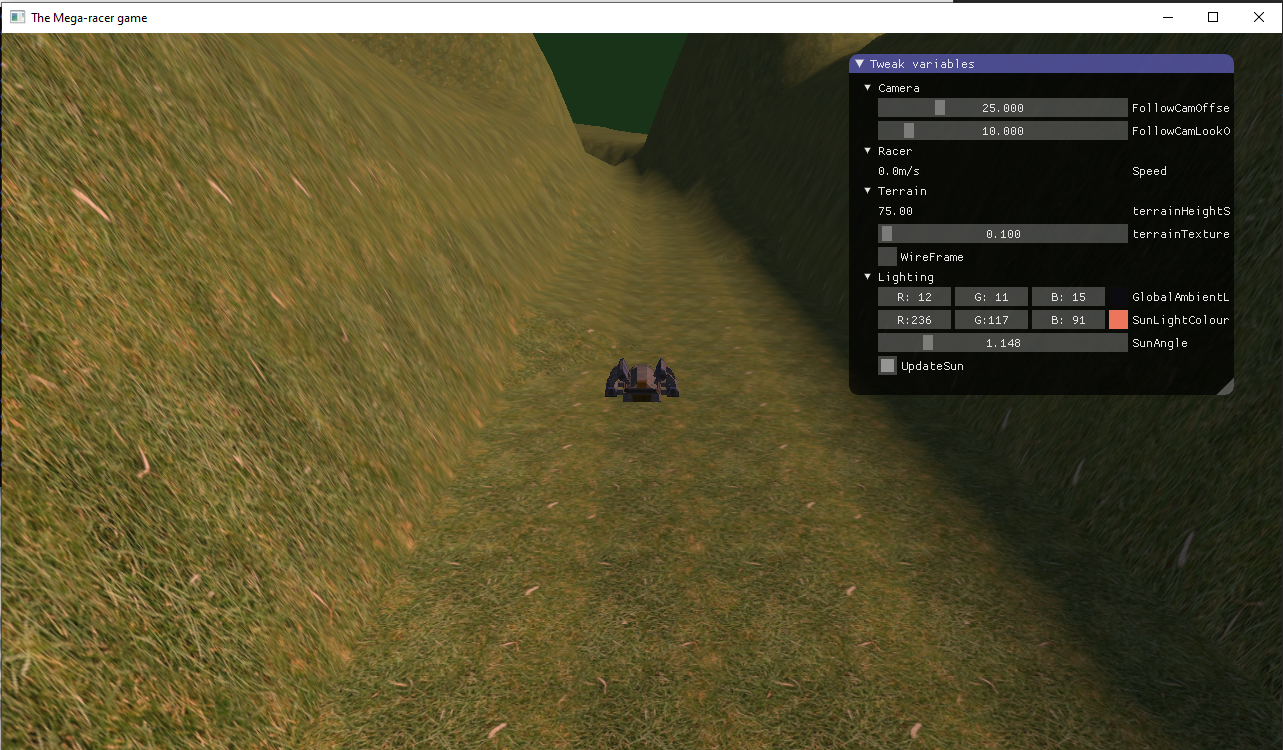
\includegraphics[width=0.49\textwidth, frame]
            {./images/mega_racer/1.5_e_1.PNG}%
        \hfill
        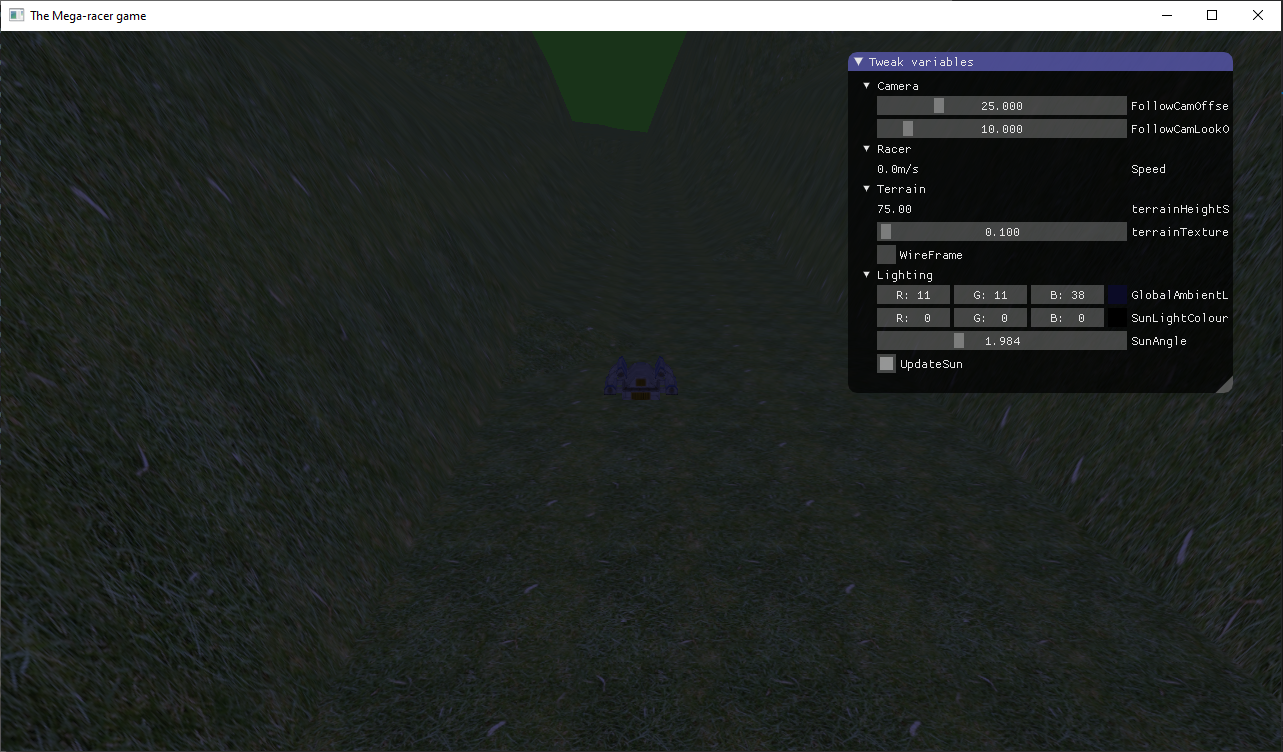
\includegraphics[width=0.49\textwidth, frame]
            {./images/mega_racer/1.5_e_2.PNG}
        }
        
        \caption{1.5 - Step 5}   
    \end{figure}

\textbf{Side notes:}
    \begin{itemize}
        \item As an aside, a slightly more advanced ambient  model, which is sometimes used for outdoor scenes is to have two colours and blend between
        them based on the orientation of the surface, such that things facing straight up get a blue ambient light (from the sky) and down a green tint (to represent grass reflecting light up). We will leave that for now though!
        \item Specular lighting
    \end{itemize}

\subsection{2.1 Improve terrain textures}

\textbf{(1) Set the high texture}
To set the high texture need to use the height and mix with the grass texture. The height is given by the vertex shader, which is the z position of the positionIn or worldSpacePosition variable. The terrainHeightScale is equivalent to Terrain.heightScale which is 75.0 and used as a scale factor to calculate the z coordinates for each vertex.
    \begin{lstlisting}[language=python]
# vertexShader:
v2f_height = positionIn.z
    -> v2f_worldSpacePosition = positionIn 

# render
terrainHeightScale = self.heightScale 
    -> heightScale = 75.0
    \end{lstlisting}

The same steps as the grass texture are followed including declaring a unit, the texture variable, binding the texture, setting the uniform value and loading the texture. However, sampling the texture is slightly different as instead of overriding the materialColour with the highColour, the texture should only appear at set heights and be blended with the grassColour.

\begin{lstlisting}[language=python]
    # terrain.py
    TU_High = 1
    highTexture = None
    
    def render():
        ....
        lu.bindTexture(self.TU_High, self.highTexture)
        lu.setUniform(self.shader, "highTexture", self.TU_High)
    
    def load():
        fragmentShader = 
            ...
            uniform sampler2D highTexture;
    
            void main():
            {   
                ????
            }
        
        self.highTexture = ObjModel.loadTexture("rock 2.png", "data", True)        
        \end{lstlisting}




...... About mix function ....
\begin{lstlisting}[language=python]
def mix(v0, v1, t):
    return v0 * (1.0 - t) + v1 * t
\end{lstlisting}




    \begin{lstlisting}[language=python]

def load():
    fragmentShader = 
        ...   
        void main():
        {   ....
            OR if (v2f_height > 50) {
            if ((v2f_height/terrainHeightScale) > 0.9) {
                vec3 highColour = texture(highTexture, 
                                    v2f_worldSpacePosition.xy 
                                    * terrainTextureXyScale).xyz;
                materialColour = mix(materialColour, 
                                    highColour, 
                                    (v2f_height/terrainHeightScale));
        }       
    \end{lstlisting}


    \begin{figure} [H]
        \centering
        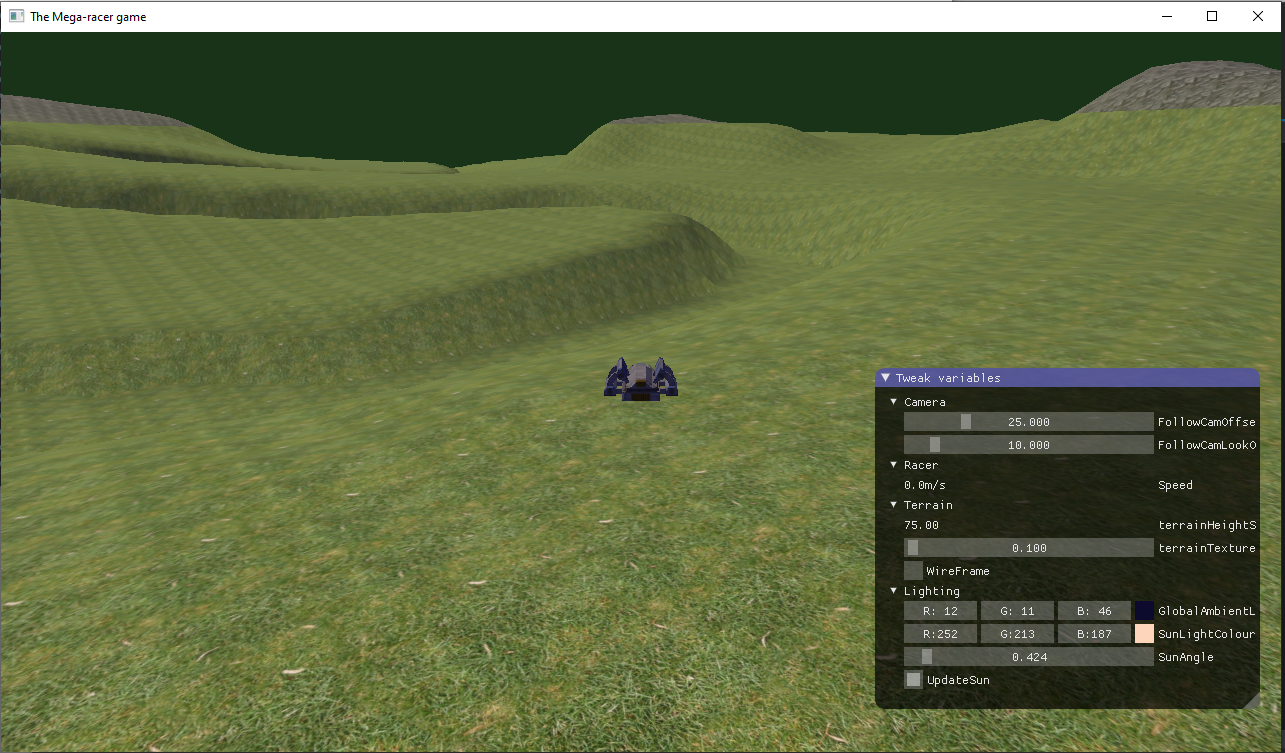
\includegraphics[width=0.8\textwidth, frame]
            {./images/mega_racer/2.1_a.PNG}
        \caption{2.1 - High Texture}   
    \end{figure}


\textbf{(2) Set the steep texture}
First thing is to get the coordinates of the normalised world space. The viewSpacePosition, viewSpaceNormal and worldSpacePosition had already been calculated so I followed the same pattern to get the worldSpaceNormal.

    \begin{lstlisting}[language=python]
    vertexShader =
        out VertexData
        {
            vec3 v2f_viewSpacePosition;
            vec3 v2f_viewSpaceNormal;
            vec3 v2f_worldSpacePosition;
            vec3 v2f_worldSpaceNormal; // NEW
        }
        void main()
        {
            v2f_viewSpacePosition = (modelToViewTransform * vec4(positionIn, 1.0)).xyz;
            v2f_viewSpaceNormal = modelToViewNormalTransform * normalIn;
            v2f_worldSpacePosition = positionIn;
            v2f_worldSpaceNormal = normalIn; // NEW
        }
    fragmentShader = 
        in VertexData
        {
            vec3 v2f_viewSpacePosition;
            vec3 v2f_viewSpaceNormal;
            vec3 v2f_worldSpacePosition;
            vec3 v2f_worldSpaceNormal; // NEW
        }
    \end{lstlisting}

    Now that the normalised world space is available to use, the slope needs to be calculated and compared to the threshold to determine when to blend the textures.

    \begin{lstlisting}[language=python]
    # terrain.py
    TU_Steep = 2
    steepTexture = None

    def render():
        ....
        lu.bindTexture(self.TU_Steep, self.steepTexture)
        lu.setUniform(self.shader, "steepTexture", self.TU_Steep)

    def load():
        fragmentShader = """
            ...
            uniform sampler2D steepTexture;

            void main()
            {....
                float slope = dot(v2f_worldSpaceNormal, vec3(v2f_worldSpaceNormal.x, 0.0, v2f_worldSpaceNormal.z));
                if (slope < 0.8) {
                    vec3 steepColour = texture(steepTexture, v2f_worldSpacePosition.xy * terrainTextureXyScale).xyz;
                    materialColour = mix(materialColour, steepColour, (v2f_height/terrainHeightScale));
            } 

        self.steepTexture = ObjModel.loadTexture("rock 5.png", "data", True)
    \end{lstlisting}

    \begin{figure} [H]
        \centering
        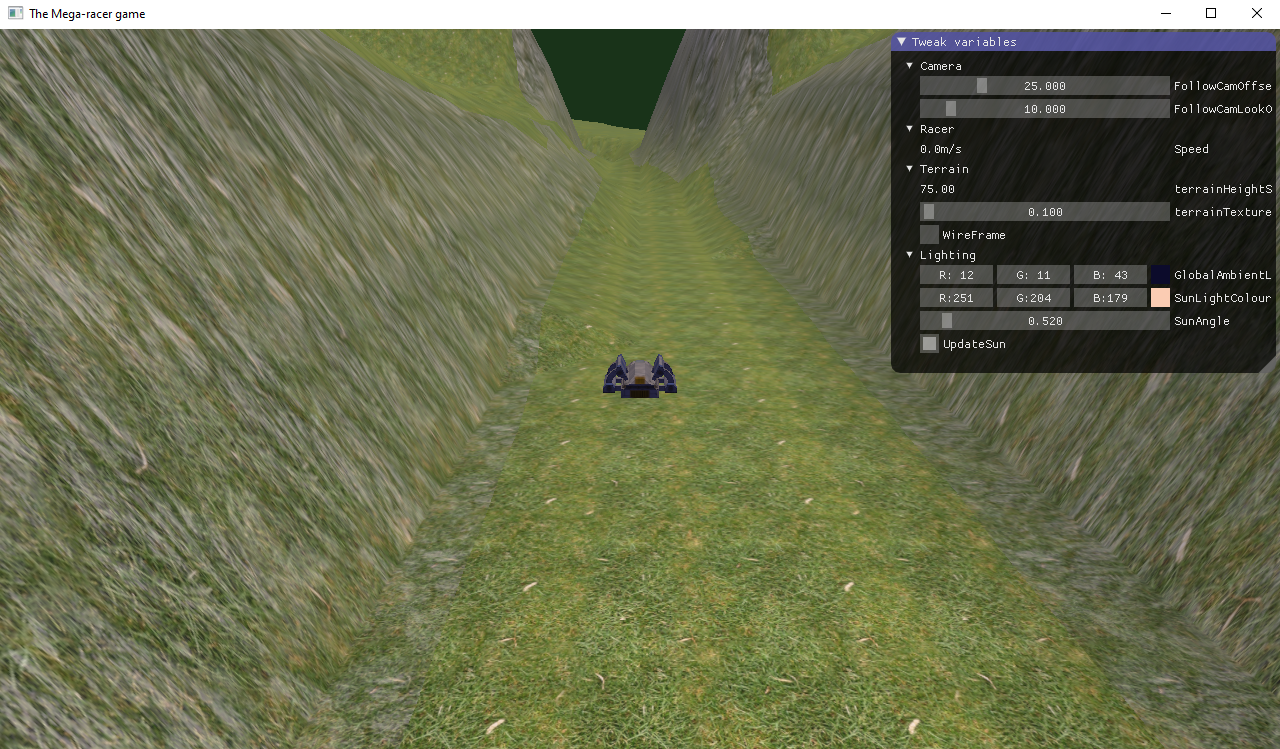
\includegraphics[width=0.8\textwidth, frame]
            {./images/mega_racer/2.1_b.PNG}
        \caption{2.1 - Steep Texture}   
    \end{figure}




\textbf{(3) Add the road}
The same steps for the other textures were then applied to roadTexture and mapTexture, except for the sampling in the main() of fragmentShader as this would be a little different. Also, when using ObjModel.loadTexture since the track image is not a SRGB file, the argument for the srgb parameter is False. 
\begin{lstlisting}[language=python]
    # terrain.py
    TU_Road = 3
    TU_Map = 4
    roadTexture = None
    mapTexture = None

    def render():
        ....
        lu.bindTexture(self.TU_Road, self.roadTexture)
        lu.bindTexture(self.TU_Map, self.roadMap)
        lu.setUniform(self.shader, "roadTexture", self.TU_Road)
        lu.setUniform(self.shader, "mapTexture", self.TU_Map)

    def load():
        fragmentShader = 
            ...
            uniform sampler2D roadTexture;
            uniform sampler2D mapTexture;

            void main():
            {   ....
                ????
            }
            }
        
        self.roadTexture = ObjModel.loadTexture("paving 5.png", "data", True)
        self.mapTexture = ObjModel.loadTexture("track_01_128.png", "data", False)
\end{lstlisting}


Since the shader doesn't have access to the type of terrain (previously relying on height and slope), the blueChannel needs to be able to be accessed so the shader knows what is considered 'road'. To be able to sample this texture the first step was to get the normalised texture coordinates. This was possible by following the similar steps to the worldSpaceNormal but with the xyNormScale and xyOffset. I knew I needed to use the xyNormScale variable instead of terrainTextureXyScale, but I wasn't sure of the purpose of offset yet. These were the last two declared variables in the vertex shader that hadn't been carried through to the fragment shader despite being declared as uniform in render() at the same time as the Texture XyScale and HeightScale.

\begin{lstlisting}[language=python]
# render()      
xyNormScale = 1.0 / (vec2(self.imageWidth, self.imageHeight) * self.xyScale);
lu.setUniform(self.shader, "xyNormScale", xyNormScale);
xyOffset = -(vec2(self.imageWidth, self.imageHeight) + vec2(1.0)) * self.xyScale / 2.0;
lu.setUniform(self.shader, "xyOffset", xyOffset);

--> 

# load()
vertexShader =
    out VertexData
    {
        vec2 v2f_xyNormScale;
        vec2 v2f_xyOffset;
    }
    void main()
    {
        v2f_xyNormScale = xyNormScale;
        v2f_xyOffset = xyOffset;
    }
fragmentShader = 
    in VertexData
    {
        vec2 v2f_xyNormScale;
        vec2 v2f_xyOffset;
    }
    \end{lstlisting}

When working on this section, it was often difficult to determine the problem, as unless the texture was declared, bound and loaded properly in the shader nothing would display. The below code is the first iteration that provided 'working' shading. The blueChannel variable followed that of the other textures, though instead of multiplying the worldSpacePosition.xy by the terrainTextureXyScale it was multiplied by the xyNormScale variable and only the z coordinate needed to be stored. The threshold of 0.9 was chosen as this produced the most accurate result. 
\begin{lstlisting}[language=python]
# terrain.py       
def load():
    fragmentShader =                 
        void main():
        {   ....
        float blueChannel = texture(mapTexture, (v2f_worldSpacePosition.xy) * v2f_xyNormScale).z;
        if (blueChannel >= 0.9) {
            vec3 roadColour = texture(roadTexture, v2f_worldSpacePosition.xy * terrainTextureXyScale).xyz;
            materialColour =  mix(materialColour, roadColour, (v2f_height/terrainHeightScale));
            }
        }
\end{lstlisting} 

When I finally did get the shader working to a point that it would display it was clear that there were still a couple of issues to resolve.

\begin{figure} [H]
    \centering
    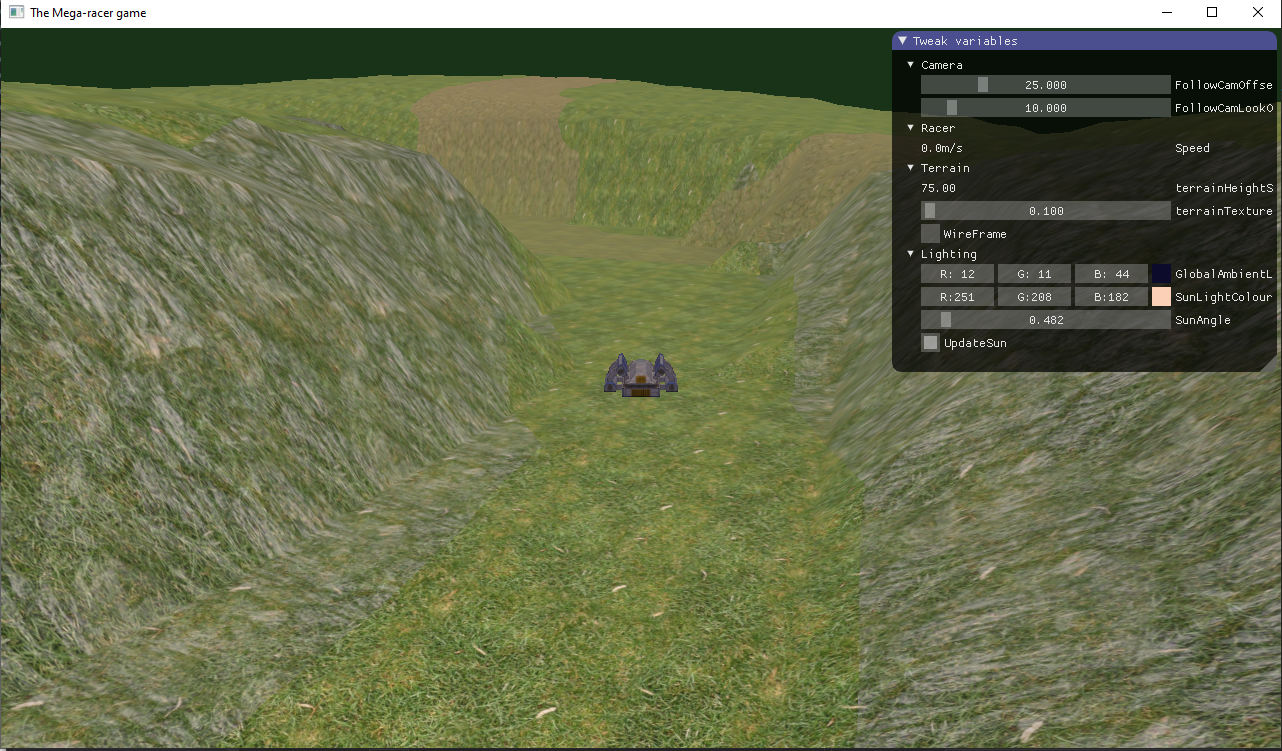
\includegraphics[width=0.8\textwidth, frame]
        {./images/mega_racer/2.1_c_1.PNG}
    \caption{2.1 - Road Texture (Mixed \& No Offset)}   
\end{figure}

\begin{enumerate}
    \item The grass texture was overtaking the blend of the pavement. This is because I mixed the roadColour with the grassColour as previously done, instead I did the same as that for the grassColour and declared the materialColour of the road to be only roadColour
    \item The road was not in the position it needed to be and was instead on the hill. This was another simple fixing by subtracting the xyOffset variable from the worldSpacePosition. After discovering this fixed the coordinates of the road I also tried mixing the road and grass colours again but the sample problem occurred.
\end{enumerate}

\begin{figure} [H]
        \makebox[\textwidth]{%
        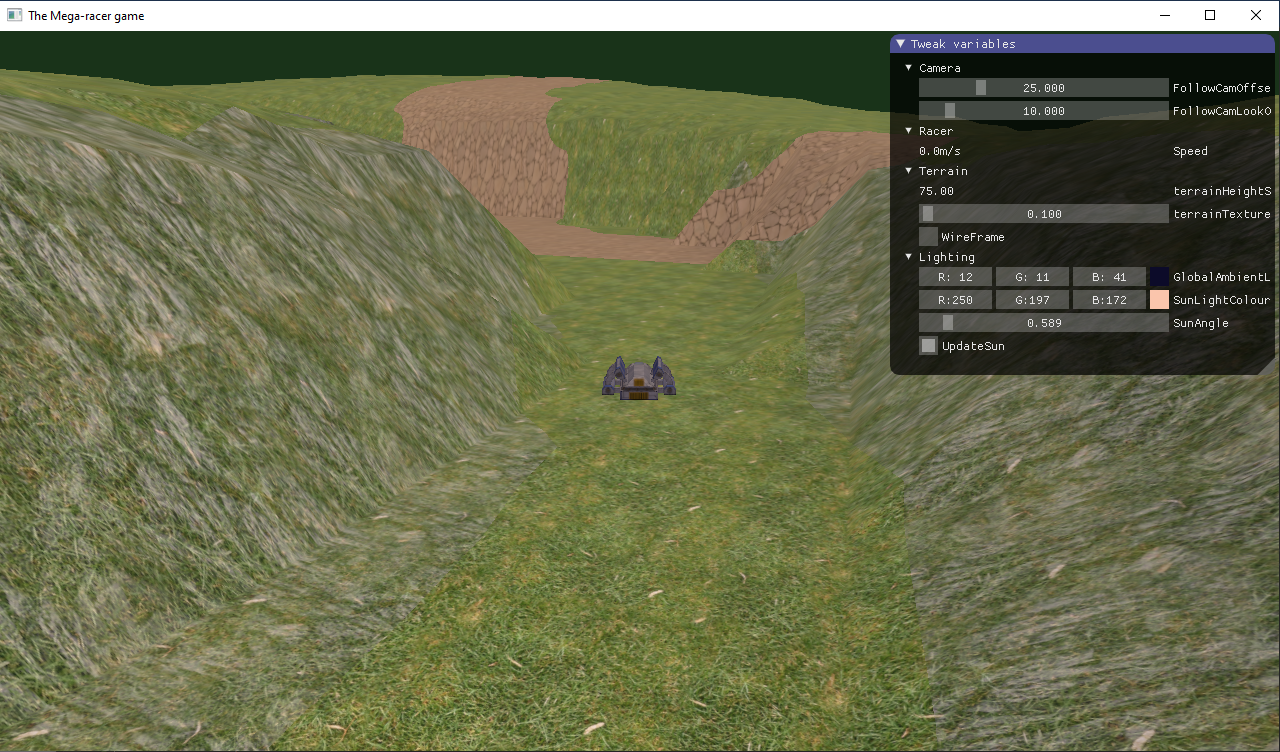
\includegraphics[width=0.49\textwidth, frame]
            {./images/mega_racer/2.1_c_2.PNG}%
        \hfill
        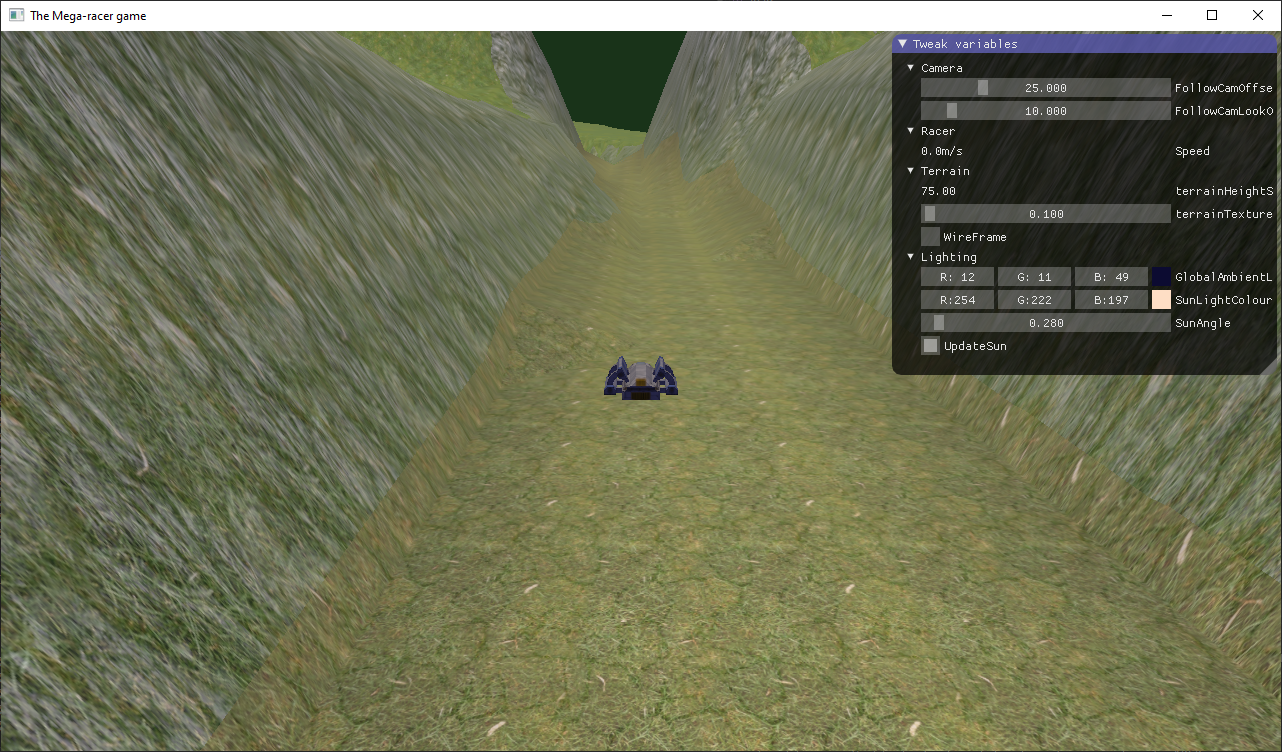
\includegraphics[width=0.49\textwidth, frame]
            {./images/mega_racer/2.1_c_3.PNG}        
        }        
        \caption{2.1 - Road Texture (Not Mixed \& No offset / Mixed \& Offset)}   
\end{figure}


After making these changes, the paving was successfully sampled and loading correctly onto the correct coordinates for the road according to the blue channel of the track.

\begin{lstlisting}[language=python]
# terrain.py       
float blueChannel = texture(mapTexture, (v2f_worldSpacePosition.xy - v2f_xyOffset) * v2f_xyNormScale).z;
if (blueChannel >= 0.9) {
    vec3 roadColour = texture(roadTexture, v2f_worldSpacePosition.xy * terrainTextureXyScale).xyz;
        materialColour = roadColour;
}
\end{lstlisting} 

    \begin{figure} [H]
        \centering
        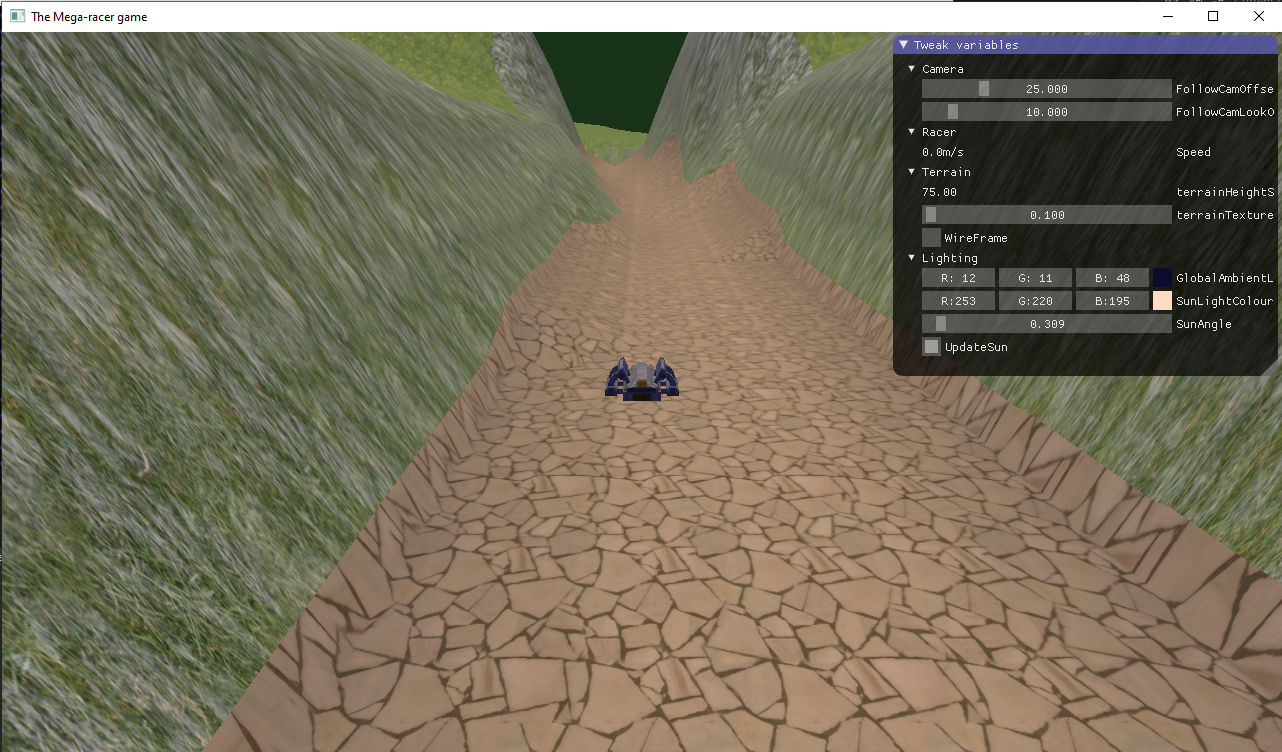
\includegraphics[width=0.8\textwidth, frame]
            {./images/mega_racer/2.1_c_final.PNG}
        \caption{2.1 - Road Texture}   
    \end{figure}

\subsection{2.2 Add Fog}

\textbf{(1) Follow the tutorial)}
Followed the tutorial exactly. Set b to 0.005 because ......

\begin{lstlisting}[language=python]
# Tutorial
vec3 applyFog( in vec3  rgb,       // original color of the pixel
                in float distance ) // camera to point distance
{
    float fogAmount = 1.0 - exp( -distance*b );
    vec3  fogColor  = vec3(0.5,0.6,0.7);
    return mix( rgb, fogColor, fogAmount );
}
-->
# mega_racer.py - Rendering system
commonFragmentShaderCode = 
    ...
    vec3 applyFog(in vec3 rgb, in float distance)
    {
        float b = 0.005;
        float fogAmount = 1.0 - exp(-distance*b);
        vec3  fogColor  = vec3(0.5,0.6,0.7);
        return mix(rgb, fogColor, fogAmount);
    }
\end{lstlisting} 

Needed to also replace the fragmentColour to call this new function:
    \begin{itemize}
        \item rgb = reflectedLight: This is currently the argument passed into toSrgb as for the 'color' parameter, so it will perform the same purpose as the 'rgb' parameter for applyFog().
        \item distance = -v2f\_viewSpacePosition.z \\      
        v2f\_viewSpacePosition = (modelToViewTransform * vec4(positionAttribute, 1.0)).xyz;
    \end{itemize}

\begin{lstlisting}[language=python]
#terrain.py
def load(...):
    ...
    fragmentShader = 
        ...
        void main()
        {
            ...
            fragmentColor = vec4(toSrgb(applyFog(reflectedLight, 
                                                    -v2f_viewSpacePosition.z)), 
                                        1.0);
        }
\end{lstlisting} 

\begin{figure} [H]
    \makebox[\textwidth]{%
    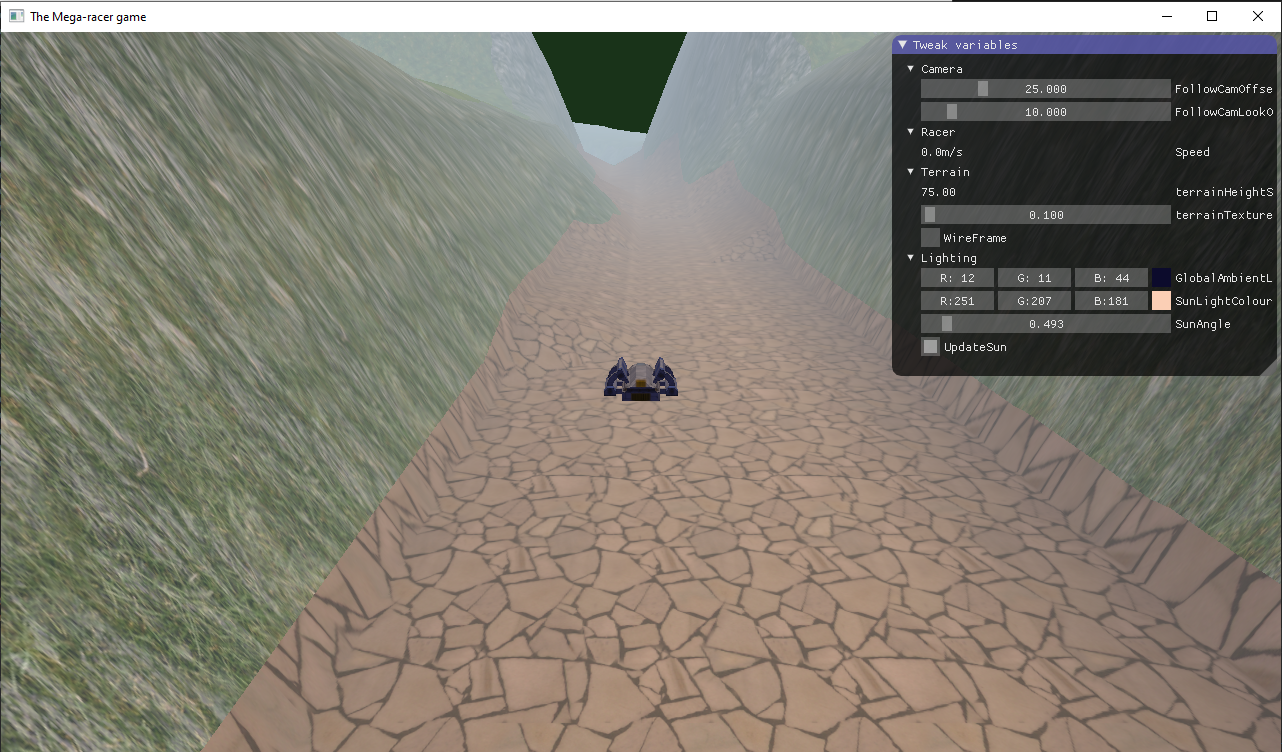
\includegraphics[width=0.49\textwidth, frame]
        {./images/mega_racer/2.2_a_1.PNG}%
    \hfill
    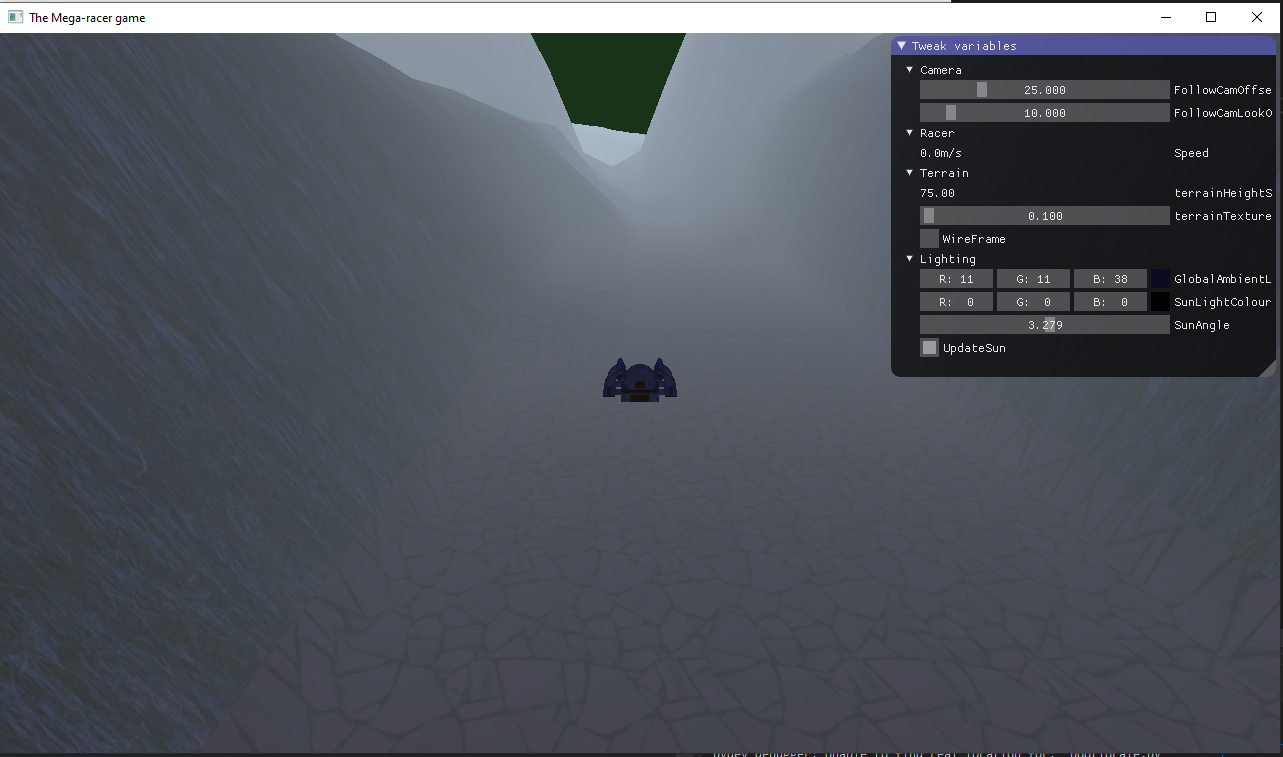
\includegraphics[width=0.49\textwidth, frame]
        {./images/mega_racer/2.2_a_2.PNG}        
    }        
    \caption{2.2 - Basic}   
\end{figure}


(2) Make colour sunLight and Ambient
The image shows how dark this makes it and project notes suggest a combination of sunLightColour and globalAmbientLight. First I tried the addition of the two
\begin{lstlisting}[language=python]
    vec3  fogColor  = (sunLightColour + globalAmbientLight)
\end{lstlisting} 

\begin{figure} [H]
    \makebox[\textwidth]{%
    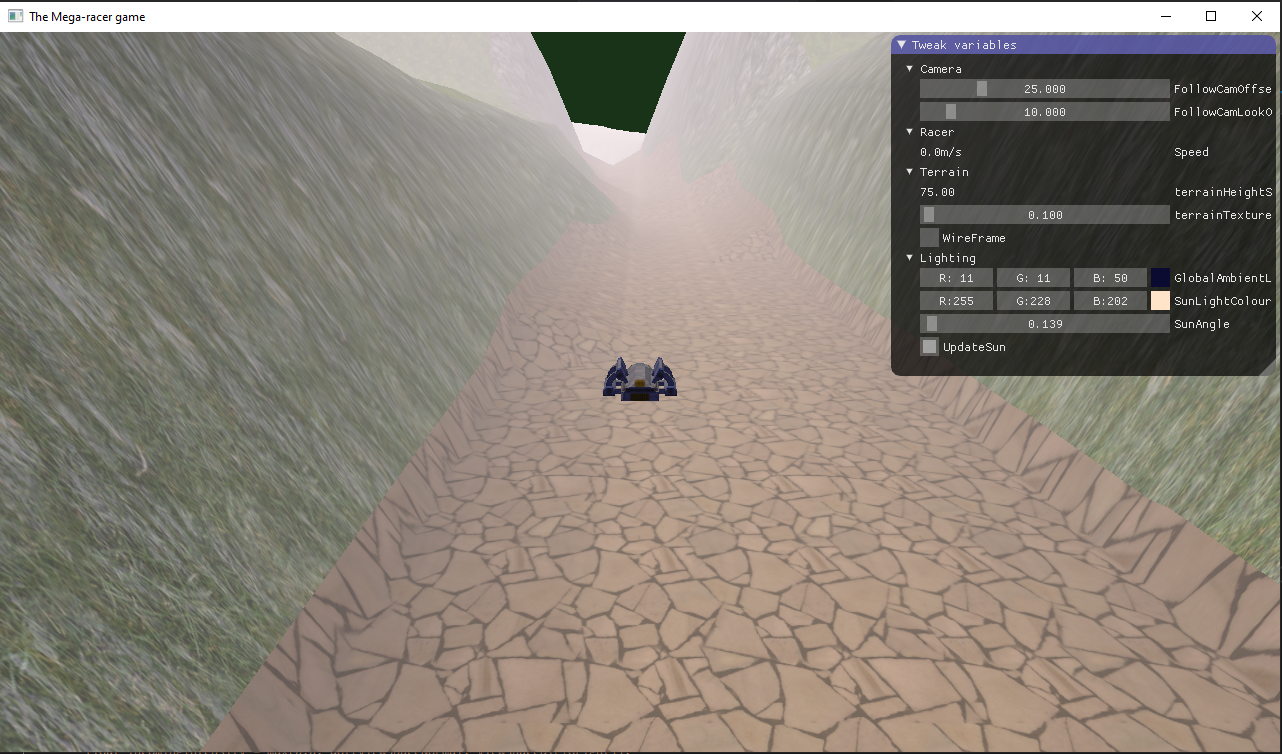
\includegraphics[width=0.49\textwidth, frame]
        {./images/mega_racer/2.2_b_1.PNG}%
    \hfill
    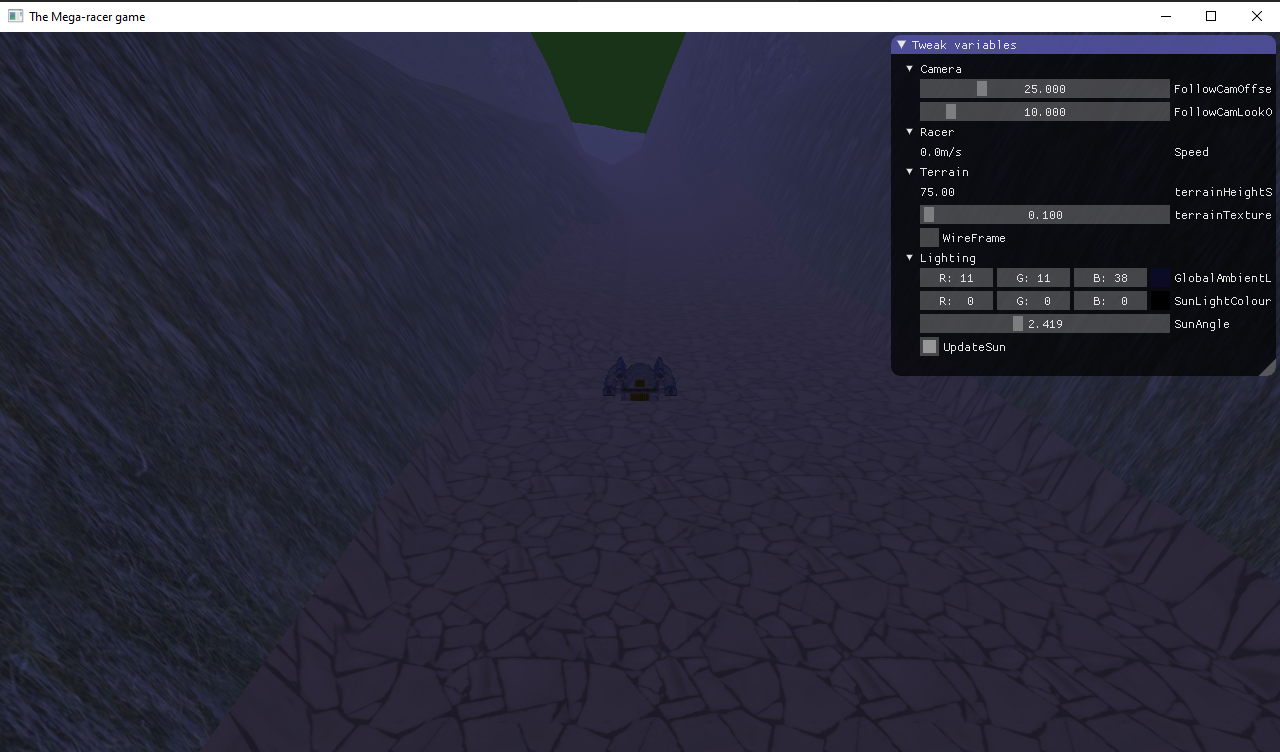
\includegraphics[width=0.49\textwidth, frame]
        {./images/mega_racer/2.2_b_2.PNG}        
    }        
    \caption{2.2 - Fog Colour (Total)}   
\end{figure}

Then I tried the average of the the two values
\begin{lstlisting}[language=python]
    vec3  fogColor  = (sunLightColour + globalAmbientLight) / 2.0
\end{lstlisting}

\begin{figure} [H]
    \makebox[\textwidth]{%
    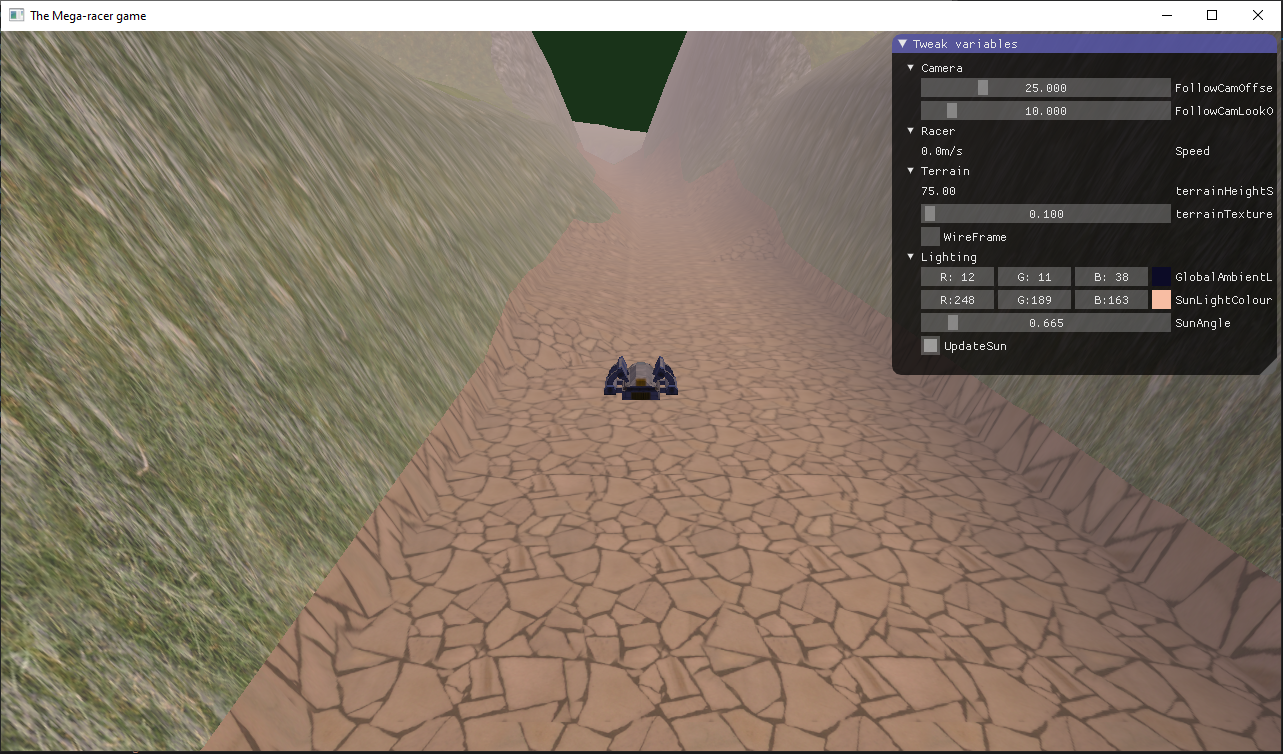
\includegraphics[width=0.49\textwidth, frame]
        {./images/mega_racer/2.2_c_1.PNG}%
    \hfill
    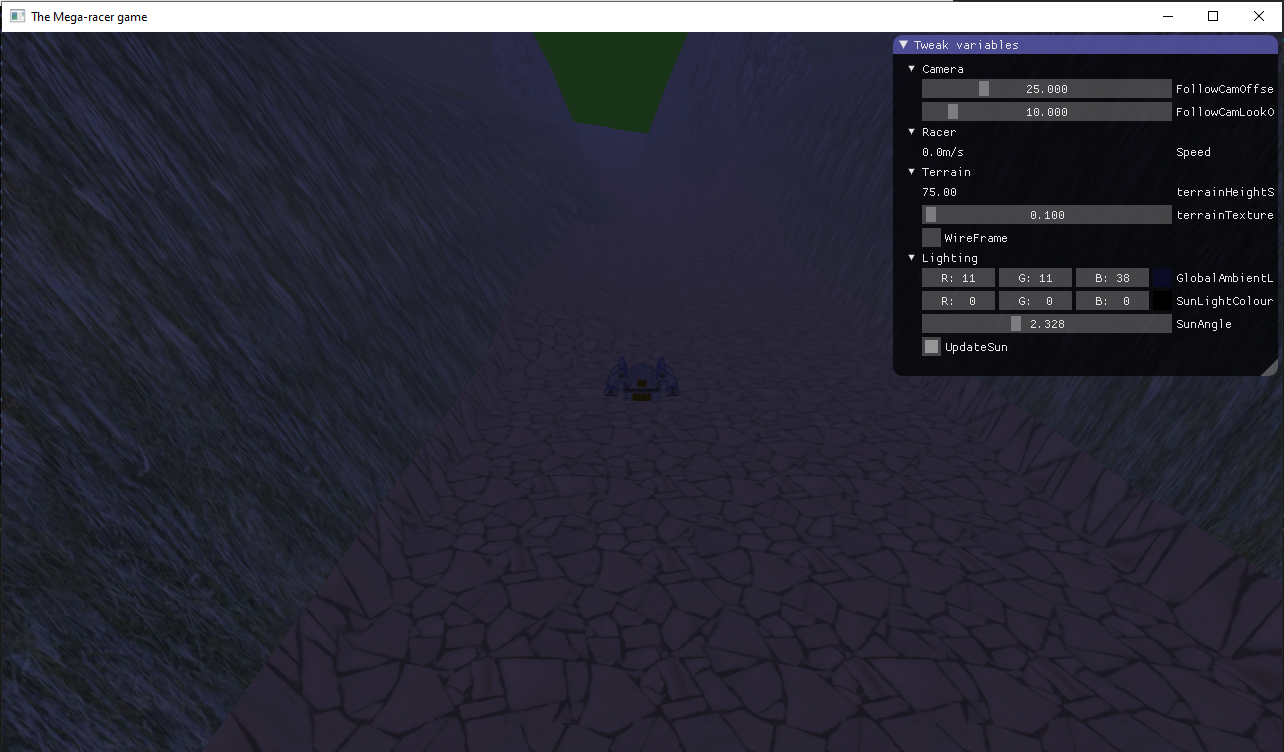
\includegraphics[width=0.49\textwidth, frame]
        {./images/mega_racer/2.2_c_2.PNG}        
    }        
    \caption{2.2 - Fog Colour (Average)}   
\end{figure}




\textbf{(3) Harder version}
This version uses height based fog.
\begin{lstlisting}[language=python]
# Tutorial
vec3 applyFog( in vec3  rgb,      // original color of the pixel
                in float distance, // camera to point distance
                in vec3  rayOri,   // camera position
                in vec3  rayDir )  // camera to point vector
{
    float fogAmount = c * exp(-rayOri.y*b) * (1.0-exp( -distance*rayDir.y*b ))/rayDir.y;
    vec3  fogColor  = vec3(0.5,0.6,0.7);
    return mix( rgb, fogColor, fogAmount );
}

-->

# mega_racer.py - Rendering system
commonFragmentShaderCode = 
    ...
    vec3 applyFog(in vec3 rgb, in float distance, in vec3  rayOri, in vec3 rayDir)
    {
        float b = 0.005;
        float c = 0.66;
        float fogAmount = c * exp(-rayOri.y*b) * (1.0-exp( -distance*rayDir.y*b ))/rayDir.y;
        vec3  fogColor  = (sunLightColour + globalAmbientLight) / 2.0;
        return mix( rgb, fogColor, fogAmount );
    }
\end{lstlisting} 

Same as before, the call to the function also needs to be updated. There are a few more variables needed as well:
    \begin{itemize}
        \item cameraPosition = vec3(worldToViewTransform[3][0],worldToViewTransform[3][1],worldToViewTransform[3][2])
        \item cameraToPointVector = normalize(positionIn - cameraPosition);
    \end{itemize}


\begin{lstlisting}[language=python]
# terrain.python
def load(...):
    ...
    vertexShader =
        \dots
        uniform mat4 worldToViewTransform;

        out VertexData
        {
            ...
            vec3 cameraPosition;
            vec3 cameraToPointVector;
        }
        void main()
        {
            ...
            cameraPosition = vec3(worldToViewTransform[3][0],worldToViewTransform[3][1],worldToViewTransform[3][2])
            cameraToPointVector = normalize(positionIn - cameraPosition);
            ...
        }
    fragmentShader = 
        in VertexData
        {
            ...
            vec3 cameraPosition;
            vec3 cameraToPointVector;
        }
        void main()
        {
            ...
            fragmentColor = vec4(toSrgb(applyFog(reflectedLight, -v2f_viewSpacePosition.z, cameraPosition, cameraToPointVector)), 1.0);
        }
\end{lstlisting} 
\begin{figure} [H]
    \makebox[\textwidth]{%
    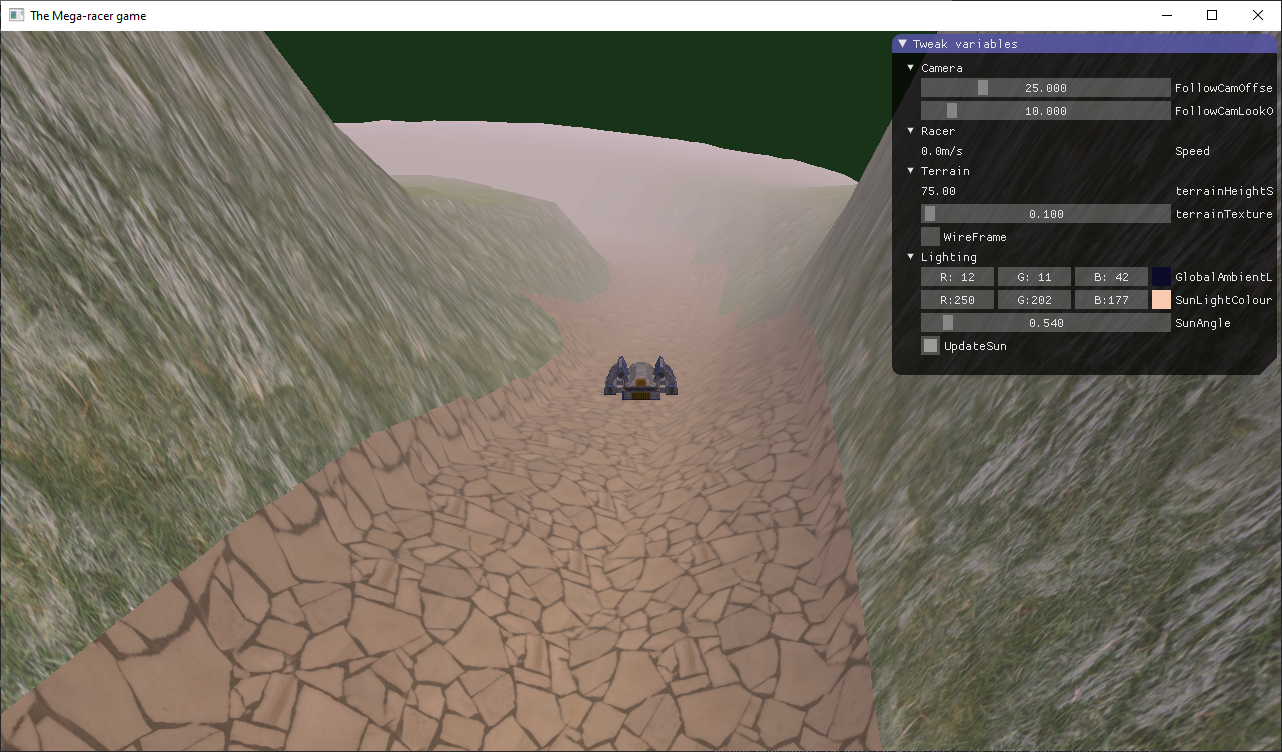
\includegraphics[width=0.49\textwidth, frame]
        {./images/mega_racer/2.2_d_1.PNG}%
    \hfill
    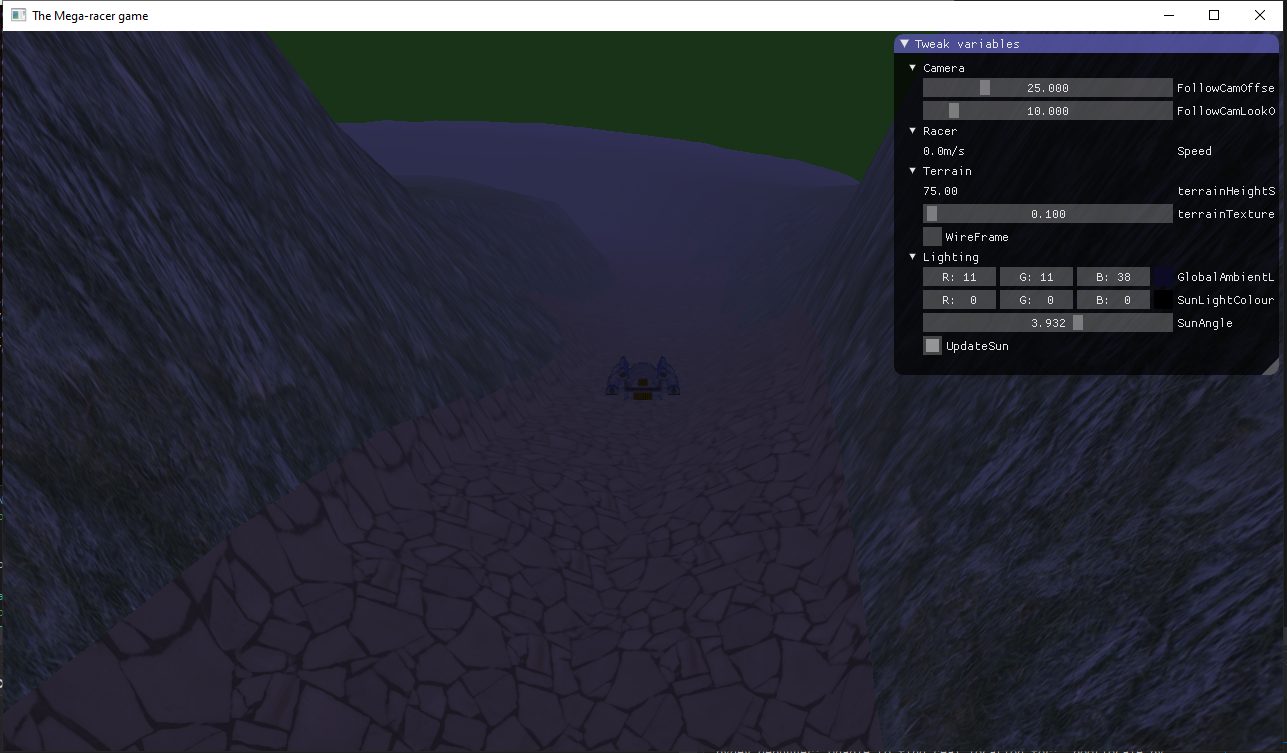
\includegraphics[width=0.49\textwidth, frame]
        {./images/mega_racer/2.2_d_2.PNG}        
    }        
    \caption{2.2 - Height Fog}   
\end{figure}


\subsection{2.3 Props}

\textbf{(1) Create the Prop class}
Followed racer.py to start of with by importing all the same libraries, creating a Prop class and copying the variables from the Racer class. From here any variables that were not required were removed (velocity, speed, maxSpeedRoad, maxSpeedRough, terrain) and new variables added (rotation). Next the render() and load() functions from the Racer class were copied (update() is not required since once created the props don't change).
    \begin{lstlisting}[language=python]
# prop.py
import libraries....

class Prop:
    position = vec3(0,0,0)    
    heading = vec3(1,0,0)
    rotation = 0.0

    zOffset = 3.0
    angvel = 2.0
    
    model = None
    \end{lstlisting}

The load() function stills needs to assign the variables of each prop instance as it did in the racer, however a few things of changed. First of all the terrain variable is no longer needed. Secondly, the position is randomised from a given list based on the prop type, as well as the rotation. This is achieved by importing the 'random' library and using choice() which randomly selects an entry from a list (https://pynative.com/python-random-choice/). Finally, the model of each unique prop should only be loaded once. The model for each prop type will be created in a prop manager class and then passed in to each instance of that prop type.
    \begin{lstlisting}[language=python]
#prop.py - Prop
import random

def load(self, model, locations):      
    self.position = random.choice(locations)
    self.rotation =random.choice(range(0,360))
    self.model = model
    \end{lstlisting}

The render() function needed to follow the same steps from Racer.render(), as well as apply the random rotation of props in the world. The only difference is that when calling drawObjModel() the modelToWorldTransform parameter is multiplied by a matrix construction function (defined in lab\_utils.py) based on the random rotation as the angle argument. 
    \begin{lstlisting}[language=python]
#prop.py - Prop
def render(self, view, renderingSystem):
    modelToWorldTransform = lu.make_mat4_from_zAxis(self.position, self.heading, [ 0.0, 0.0, 1.0 ])
    rotationMatrix = lu.make_rotation_y(self.rotation)
    renderingSystem.drawObjModel(self.model, modelToWorldTransform * rotationMatrix, view)
    \end{lstlisting}
 
\textbf{(2) Create the PropManager class}
Now, that the Prop class has been created the next step was to create a class to manage all of the prop instances; PropManager. To start the required variables were declared. For each prop type there needed to be a maximum number of instances, a list to keep track of the instances, a single model.
    \begin{lstlisting}[language=python]
# prop.py
class PropManager: 
    treeMax = 50
    treeList = []
    treeModel = None

    rockMax = 20
    rockList = []
    rockModel = None
    \end{lstlisting} 

Now to create the instances of each prop type and save them in a global list (treeList or rockList). The process is the same for all prop types so a general function, loadPropList(), creates the instances for the prop type and fills the list. For each prop type, there are max number of instances (propMax). Each of these instances uses a single model of the prop type (propModel) with a position from the designated list for that prop type (propLocations). The instance is then appended to the relevant list for easier access (propList). 
    \begin{lstlisting}[language=python]
# prop.py - PropManager
def loadPropList(self, propModel, propMax, propLocations):
propList = []
i = 0
while i < propMax:
    prop = Prop()
    prop.load(propModel, propLocations)
    propList.append(prop)            
    i += 1
    print(prop.position)
return propList
    \end{lstlisting} 

This function is called for each prop type, with their specific values, and assigned to the relevant prop type list in loadAllProps(), after first creating the unique model for each prop type in loadAllProps(). This means the model for each prop is created only once and all instances share the same model (i.e. textures, vector data, etc). 
    \begin{lstlisting}[language=python]
# prop.py - PropManager 
def loadAllProps(self, terrain): 
    # Load trees
    self.treeModel = ObjModel("data/trees/birch_01_d.obj")
    self.treeList = self.loadPropList(self.treeModel, self.treeMax, terrain.treeLocations)
    # Load rocks
    self.rockModel = ObjModel("data/rocks/rock_01.obj")
    self.rockList = self.loadPropList(self.rockModel, self.rockMax, terrain.rockLocations)
    \end{lstlisting}


With the PropManager defined the props can now be loaded in the world. The PropManager class needs to be imported and the variable created. Then, below were the g\_racer and g\_terrain are being assigned as instances of their corresponding class' and loaded, the same needs to be done for the props as g\_props.

    \begin{lstlisting}[language=python]
#mega_racer.py
from prop import PropManager
...
g_props = None
....
g_props = PropManager()
g_props.loadAllProps(g_terrain)
    \end{lstlisting}


\textbf{(3) Render all props}   
    \begin{lstlisting}[language=python]
# prop.py - PropManager 
def renderAllProps(self, view, renderingSystem):
    for prop in self.allProps:
        prop.render(view, renderingSystem)
    \end{lstlisting}

Again in the same area as the g\_racer and g\_terrain variables are rendered this render function will be called. 
    \begin{lstlisting}[language=python]
    #mega_racer.py    
    def renderFrame(...):
        ...
        g_props.renderAllProps(view, g_renderingSystem)
    \end{lstlisting}

    \begin{figure} [H]
        \centering
        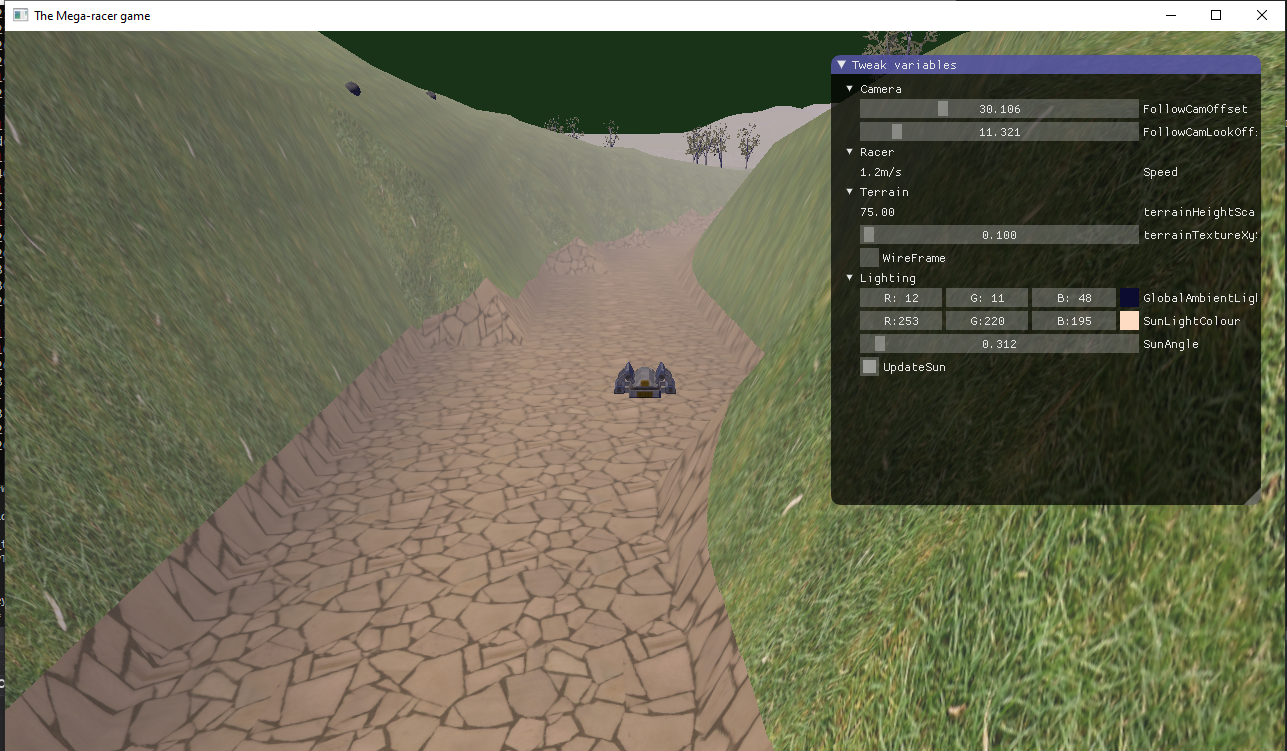
\includegraphics[width=0.8\textwidth, frame]
            {./images/mega_racer/2.3.PNG}  
        \caption{2.3 - Props (trees and rocks)}   
    \end{figure}



\section{Olympic Stadium}
- Rename mega\_racer.py to olympic\_stadium.py


\subsection{Track}

Scale by using dimensions of \href{https://www.dimensions.guide/element/track-and-field-400m-running-track}{athletic track}



\subsection{Props}

In the process of changing elements in the mega\_racer world to reflect an Olympic stadium all of the object models (.obj and .mtl) needed to be either created or modified in blender. This was either because an appropriate free .obj file could not be found or was scaled incorrectly, and/or the .mtl file was missing or not correct. Some basics that needed to be learned to get started was scaling (\href{https://www.youtube.com/watch?v=FPp3ClfDYqI}{tutorial}) and rotating(\href{https://www.youtube.com/watch?v=NUy2O13QH68}{tutorial}).


\subsubsection{Athlete}
Instead of a race car driving around the track, I wanted to replace it with an athlete. A person is quite a complicated model to make from scratch so I looked to source a premade .obj model of a basic person. I decided to go with \href{https://free3d.com/3d-model/male-base-mesh-6682.html}{this} free basic mesh male model uploaded by Paul Chen on free3d.com. The model is in a basic standing position with no texturing. For a more realistic model for the stadium, the model needed to be scaled appropriately and posed in a running position. Importing the .obj file in blender and following \href{https://www.youtube.com/watch?v=XHa2Y8zjtZQ}{this} basic rigging tutorial on YouTube by PIXXO 3D, a meta-rig was set up for the model. This basically entails lining up a bone framework, like a skeleton, to the model. One of the errors I ran into was moving one of the spine bones on accident so that it was detached disallowing the meta-rig from generating, however it was solved from \href{https://blender.stackexchange.com/questions/169555/rigify-error-bone-cannot-connect-chain-bone}{this} post through the blender forum.
    \begin{figure} [H]
        \makebox[\textwidth]{%
        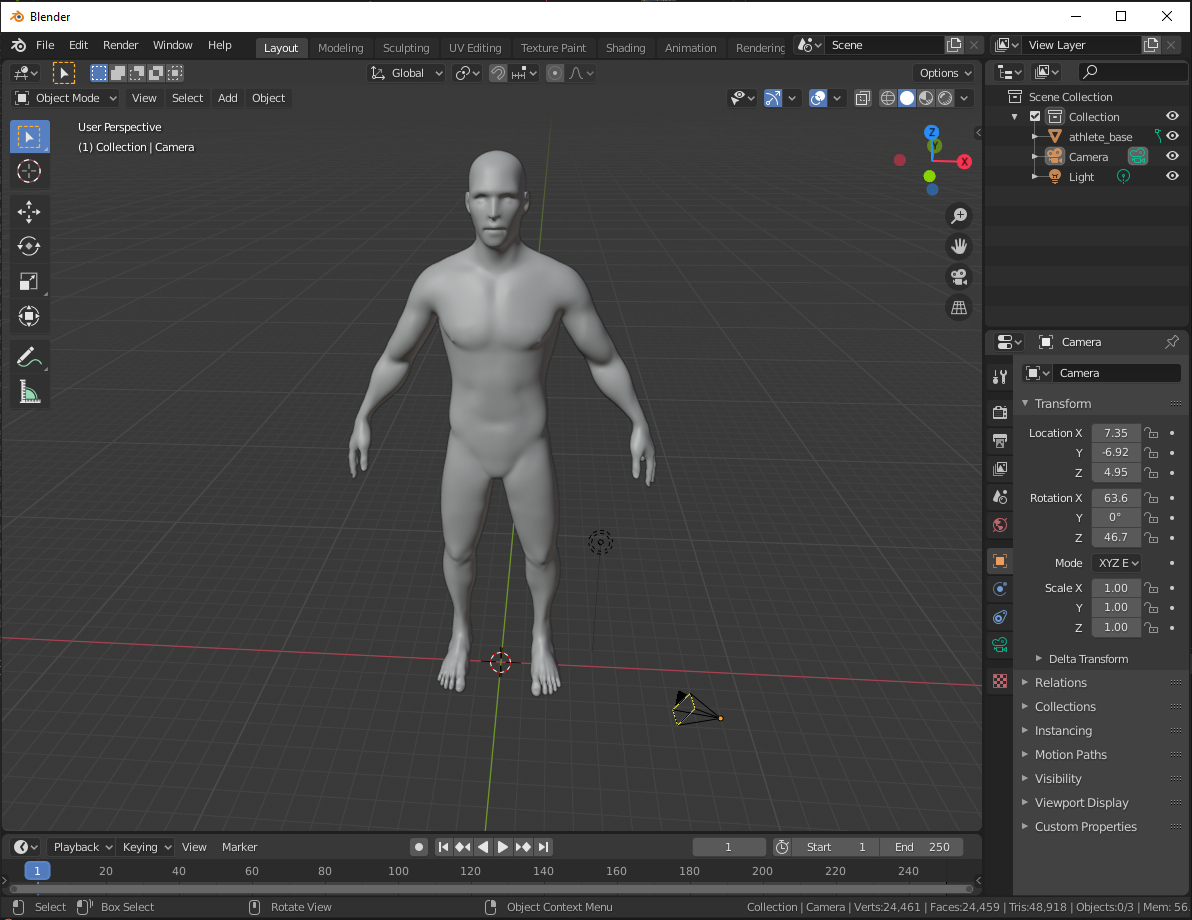
\includegraphics[width=0.49\textwidth, frame]
            {./images/olympics/athlete_blend_base.PNG}%
        \hfill
        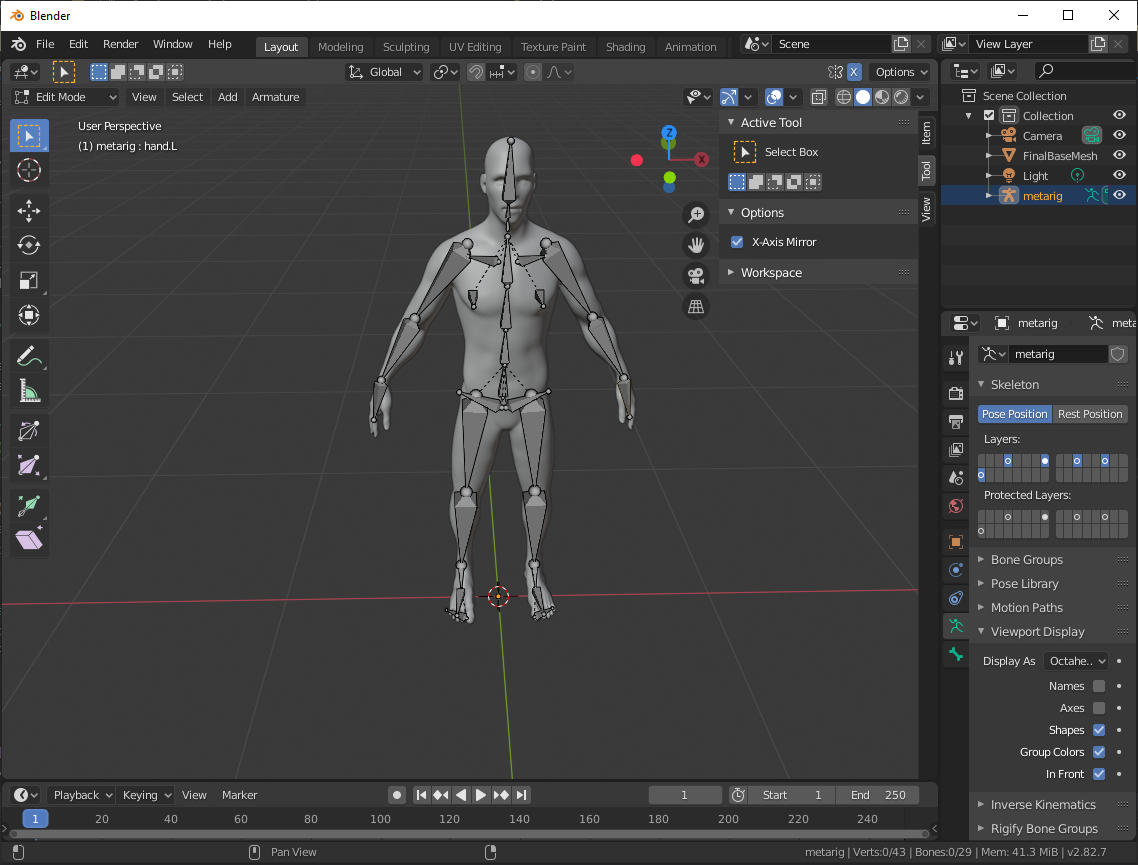
\includegraphics[width=0.49\textwidth, frame]
            {./images/olympics/athlete_blend_metarig.PNG}        
        }        
        \caption{Racer - Blender - Base \& Rig}   
    \end{figure}

Using this meta-rig, blender has a built-in feature that creates a rig that can be used to move the 'bones' around to place the model into poses. For my model, I needed to life one leg backward from the knee and point the foot down, and slightly lift the other foot and bend the knee slightly forward. The arms were moved in the same fashion with one arm back and the hand pointing down and the other arm forward with bend elbow and hand pointing up. Essentially, this put the model in a running pose.
    \begin{figure} [H]
        \makebox[\textwidth]{
        \centering
        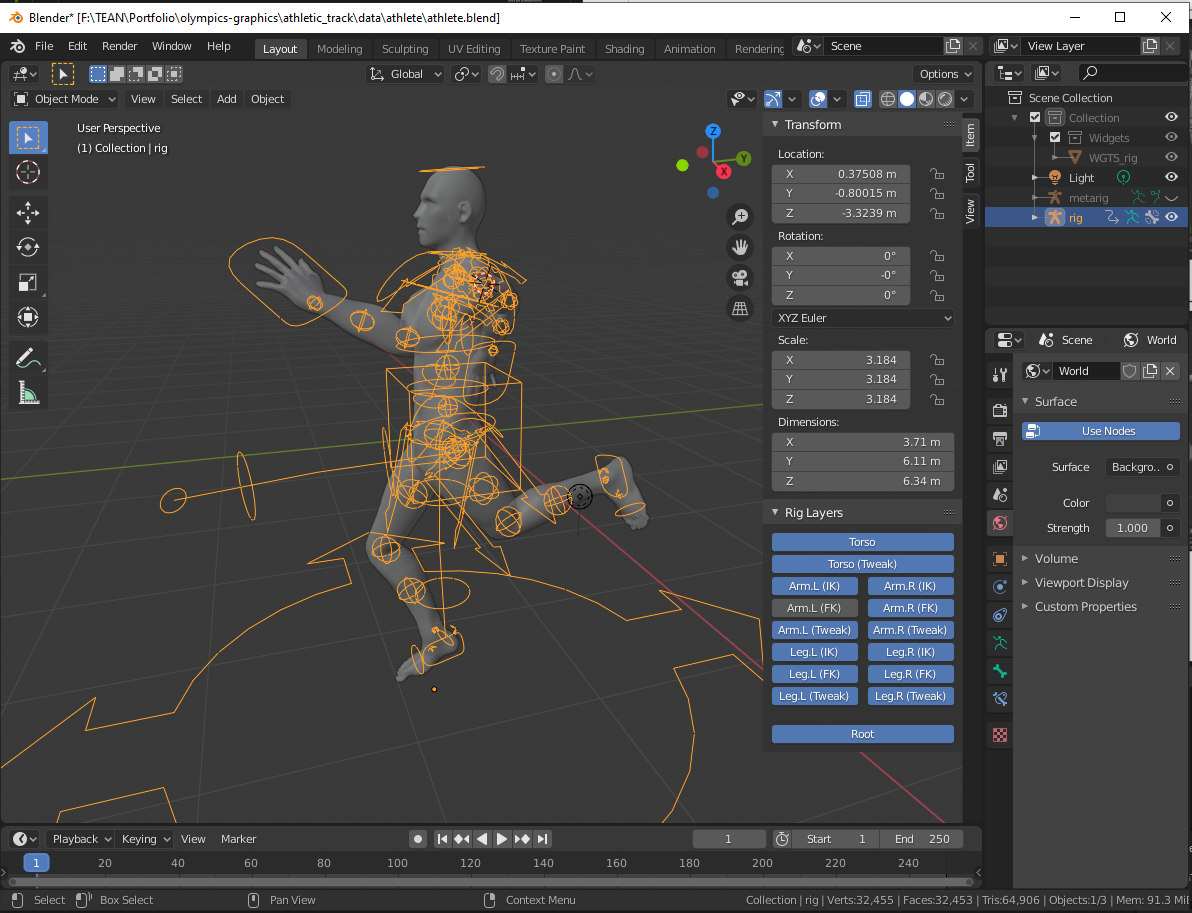
\includegraphics[width=0.49\textwidth, frame]
            {./images/olympics/athlete_blend_rig2.PNG}
        \hfill
        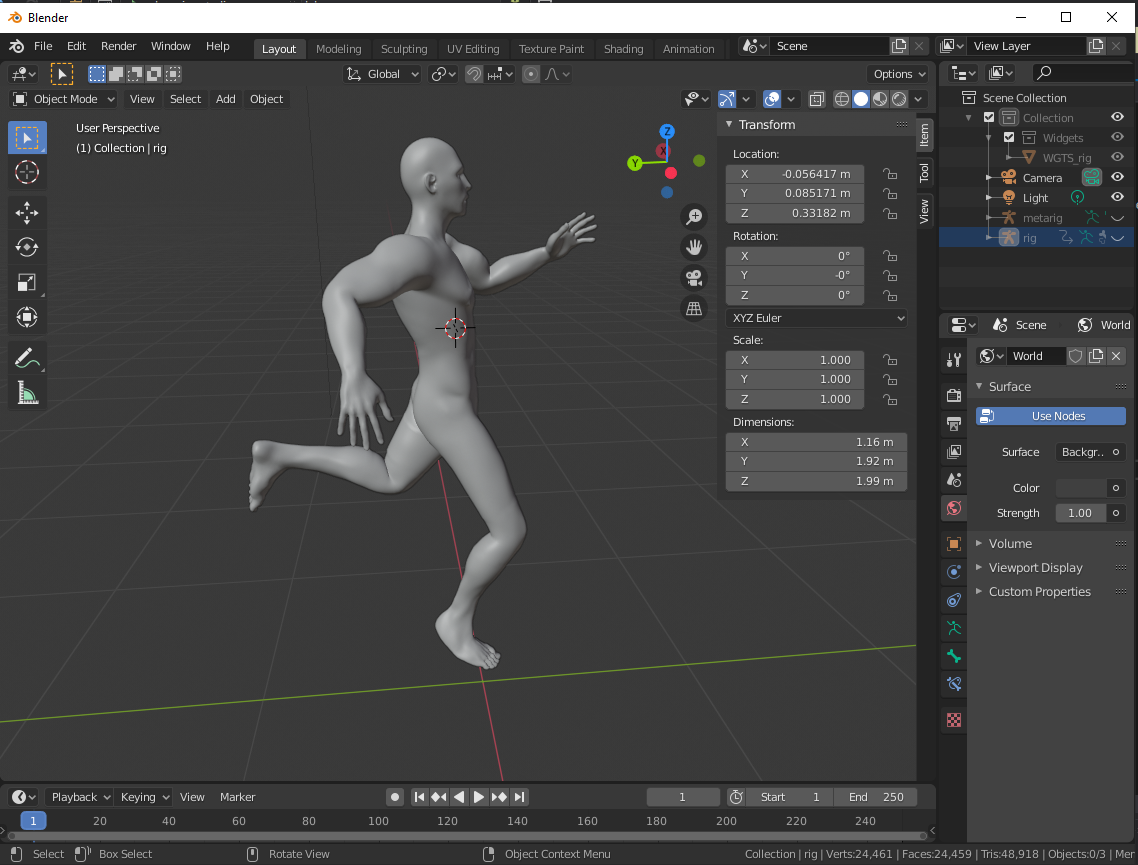
\includegraphics[width=0.49\textwidth, frame]
            {./images/olympics/athlete_blend_pose.PNG}        
        }        
        \caption{Racer - Blender - Posing}   
    \end{figure}

Now that the athlete was in the running position, some texturing needed to be added. Sourcing images from Google, I found some textures that were appropriate for an athlete including Lycra and breathable material. However, since the model was set as all one material I learnt from \href{https://www.youtube.com/watch?v=afjGodkdp4U}{this} tutorial on YouTube from Jayanam, that I needed to use vertex groups in order to separate them into different sections. In this step, I would have liked to have learn to extrapolate the areas to give them definition and shape the areas to look as they should i.e. make the feet look like shoes. For this basic model, I decided to just colour the separate areas using the image textures I had found. After creating the groups I was able to colour them separately assigning the different materials to the groups as done by \href{https://www.youtube.com/watch?v=ZWJB7HaKJZY}{this} tutorial from Weisbrod Imaging on YouTube.
    \begin{figure} [H]
        \makebox[\textwidth]{%
        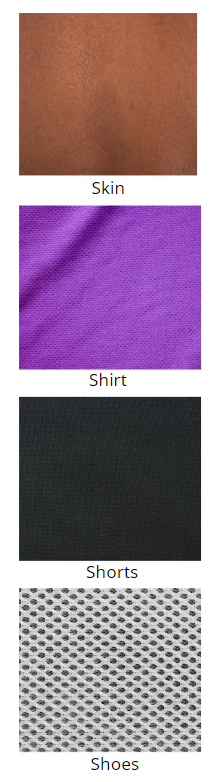
\includegraphics[width=0.15\textwidth, height=0.41\textheight, frame]
            {./images/olympics/athlete_textures.PNG}%
        \hfill
        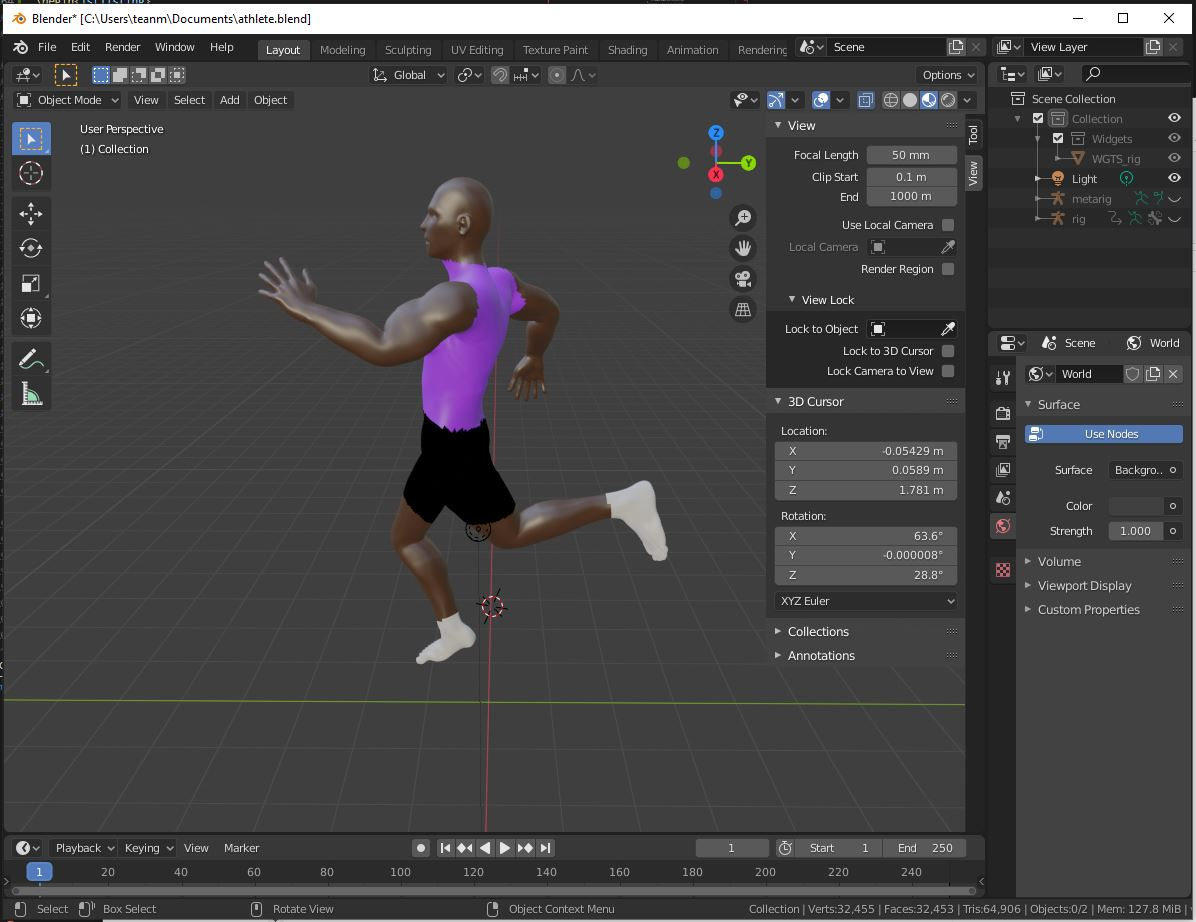
\includegraphics[width=0.8\textwidth, frame]
            {./images/olympics/athlete_blend_colour.jpg}        
        }        
        \caption{Racer - Blender - Colour}   
    \end{figure}

The athlete was coming together! However, I really didn't like the dodgy colouring attempt so I decided to try and add clothing for more realistic texturing. I found the following free clothing models on turbosquid.com:
\begin{itemize}
    \item \textbf{Men Avatar Vest} by swatishr13: href{https://www.turbosquid.com/FullPreview/Index.cfm/ID/1557152}{This} model was imported with no colouring associated. The trims on the sleeve were set as white and the main colour used the same 'top' texture as in the previous colouring. 
    \item \textbf{short pants} by sazandra: \href{https://www.turbosquid.com/FullPreview/Index.cfm/ID/1434049}{This} file was able to be imported with all textures correctly. Since the model was in a running position, the pants were the wrong shape however the model used a mirror modify so I was able to split the model and just have half of the pants. This half of the pants were used as is and then duplicate was made with a mirror image of the local x and y coordinates that could be set at the right shape for the runner.
    \item \textbf{shoe} by Bruno Dalla: \href{https://www.turbosquid.com/FullPreview/Index.cfm/ID/1217043}{This} model is of a single show so a duplicate mirrored on the local x was created. The associated texturing for this model didn't load correctly so the above 'shoe' texturing was used except for a trim around the bottom the same colour as the top.
\end{itemize}


\begin{figure} [H]
    \centering
    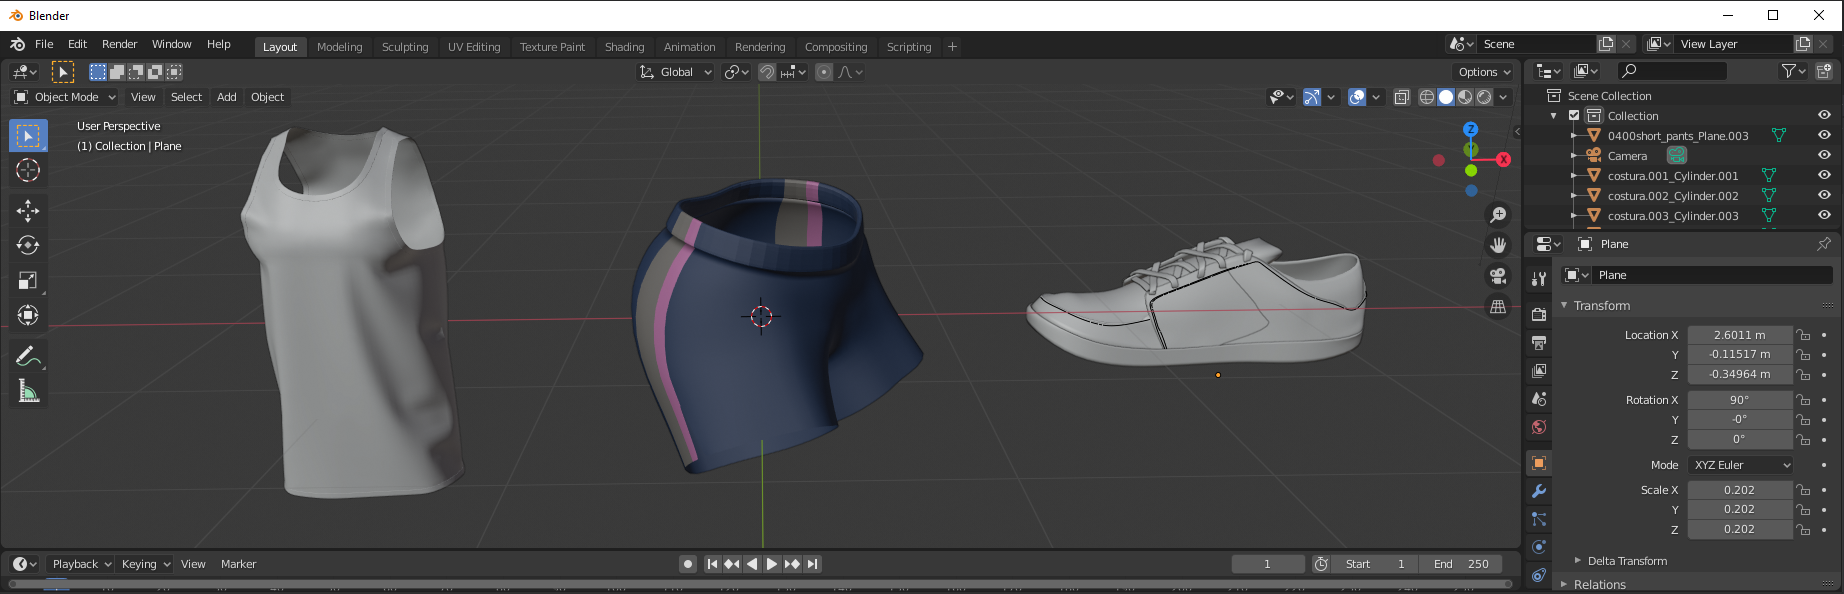
\includegraphics[width=0.9\textwidth, frame]
        {./images/olympics/athlete_clothes_base.PNG}
    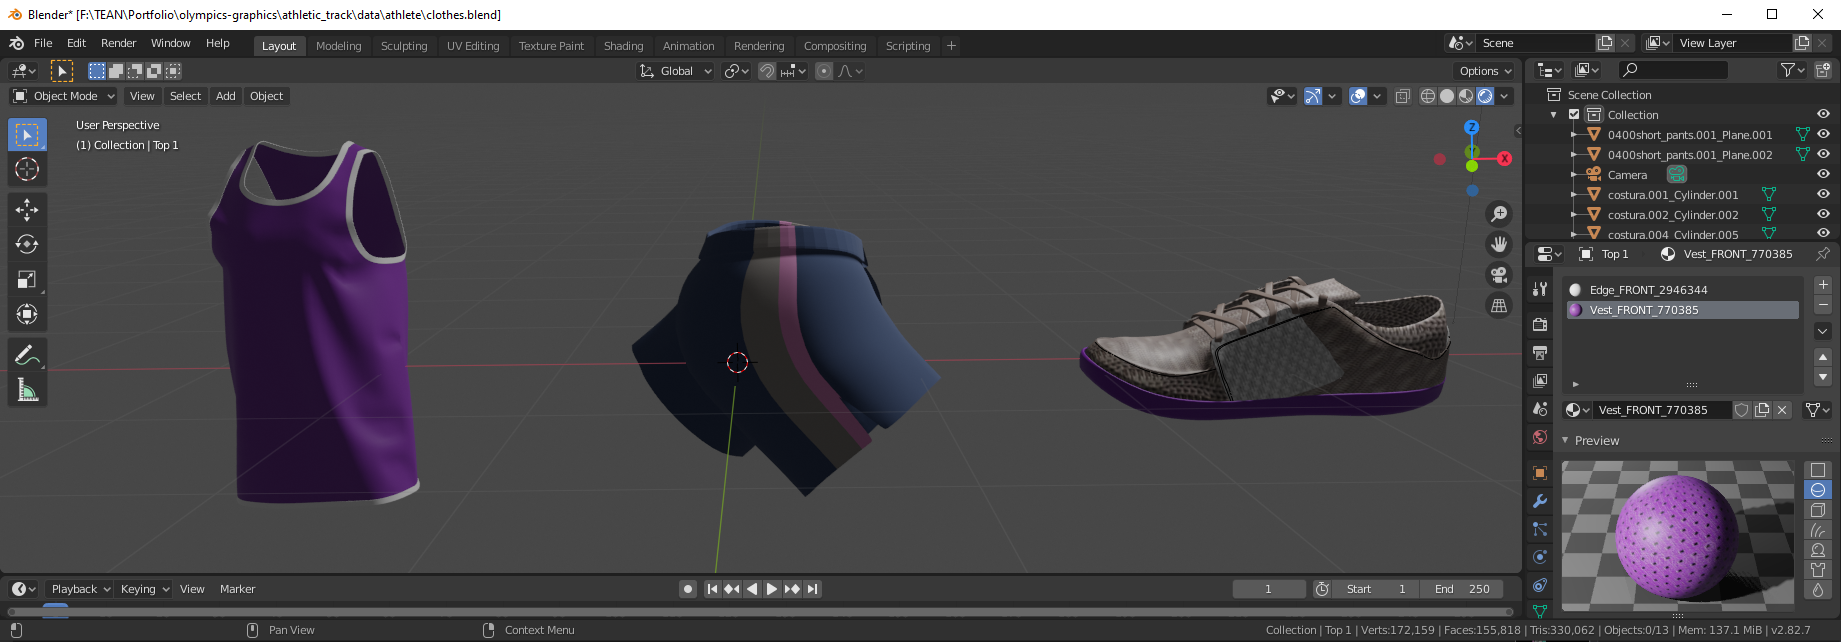
\includegraphics[width=0.9\textwidth, frame]
        {./images/olympics/athlete_clothes_colour.PNG}    
    \caption{Racer - Blender - Clothes}   
\end{figure}

Now I have a posed human model with clothes. The next step would be to add skin texturing and more human features. This was a level of detail that was beyond my ability for this project. Perhaps another time.
\begin{figure} [H]
    \centering
    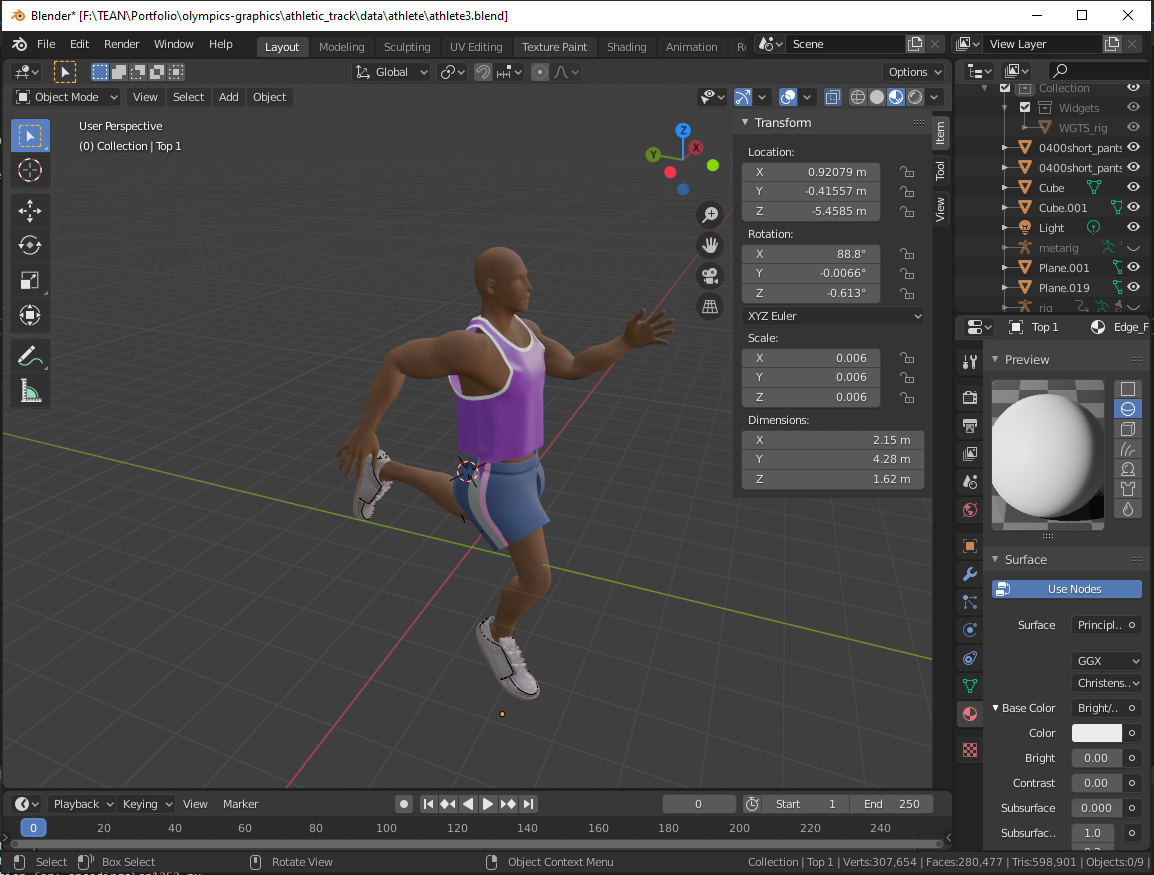
\includegraphics[width=0.8\textwidth, frame]
        {./images/olympics/athlete_blend_clothes.PNG}  
    \caption{Racer - Blender - Final}   
\end{figure}


\subsubsection{Rings}
It wouldn't be the Olympics without the iconic Olympic rings. Originally I sourced \href{https://www.cgtrader.com/free-3d-models/architectural/other/3d-olympic-rings}{this} model on cgtrader.com, however after trying to open it in blender not only were the set materials not working from the .mtl file but also the rings were connected and overlapping so I wasn't able to separate them out to colour them differently. They seemed simple enough to make myself so following \href{https://www.youtube.com/watch?v=yaWl43Z0QQk}{this} time-lapse video and sourcing my own textures for the rings I made a new model that could be used on the centre area of the stadium. Each ring is a torus that was reshaped slightly, coloured with the textures and then overlapped with the two bottom rings in front. 
    \begin{figure} [H]
        \makebox[\textwidth]{%
        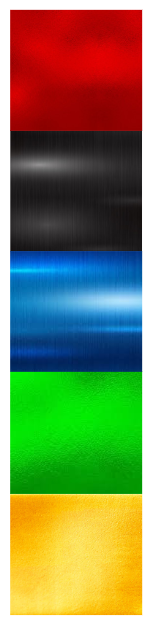
\includegraphics[width=0.15\textwidth, height=0.41\textheight, frame]
            {./images/olympics/rings_textures.PNG}%
        \hfill
        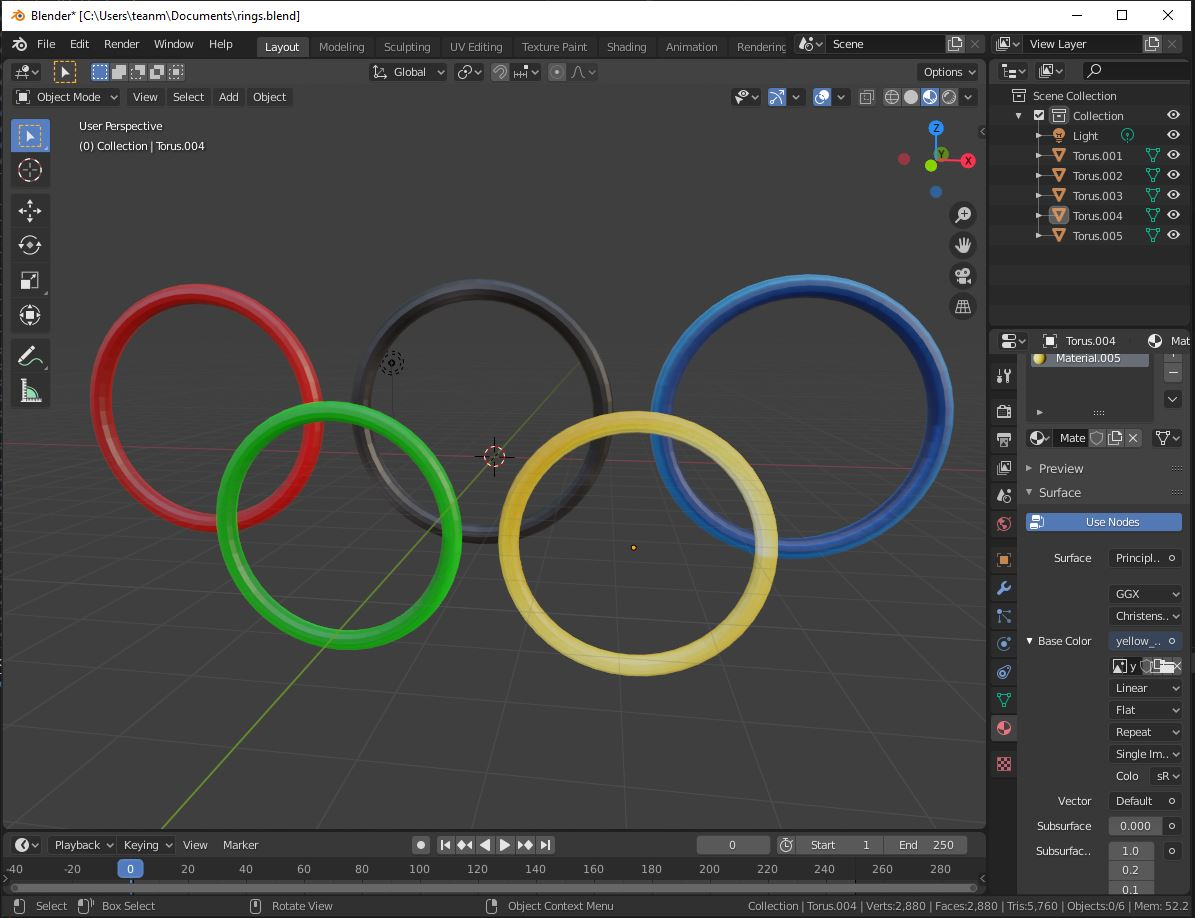
\includegraphics[width=0.8\textwidth, frame]
            {./images/olympics/rings_blend.jpg}        
        }        
        \caption{Props - Rings}   
    \end{figure}

\subsubsection{Cones}
To demonstrate props that would be repeated on a large scale, I decided to place safety cones around the inside of the middle area of the stadium. Similar to the Olympic rings, I found \href{https://www.cgtrader.com/free-3d-models/exterior/street/cone-2b4a9172-7afb-4611-8e23-bdac1afe0b87}{various} models on cgtrader.com but the .mtl file was not correct for any of them, so I decided to create my own cones. Following \href{https://www.youtube.com/watch?v=vQ_1HU_-BJM}{this} tutorial I was able to make a realistic traffic safety cone. The cone started as a cylinder, the top was reshaped for the cone appearance, the lip on the top was created, a base added, the strips added using loop cuts and finally the colouring applied.
    \begin{figure} [H]
        \centering
        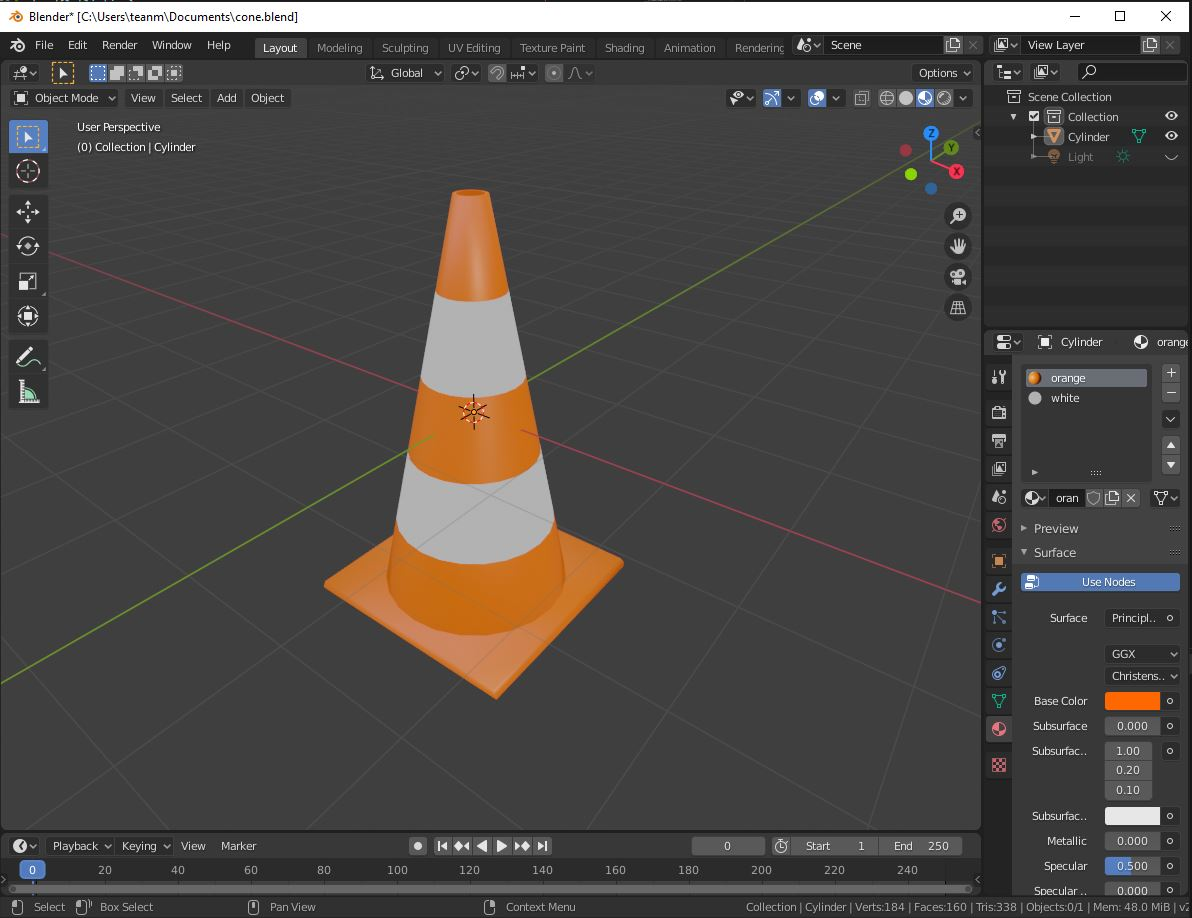
\includegraphics[width=0.8\textwidth, frame]
            {./images/olympics/cone_blend.jpg}
        \caption{Props - Cone}   
    \end{figure}


\subsubsection{Podium}
\begin{lstlisting}
    Podium:
https://xotv.me/channels/219-proseso/vod_videos/3317-how-to-model-a-winners-podium-in-blender-lesson-2 

https://www.cgtrader.com/free-3d-models/sports/equipment/sport-final-ceremony-podium

Seperate:
https://www.youtube.com/watch?v=U3J-oYFdyqQ
\end{lstlisting}






\begin{lstlisting}[language=python]
#mega_racer.py
g_props = PropManager()
propTypes = [['cone', 50, g_terrain.treeLocations], ["rings", 2, g_terrain.rockLocations]]
g_props.loadAllProps(propTypes)

#prop.py
class PropManager: 
    propTypes = []
    allProps = []    

    def loadProp(self, propType):
        propModel = ObjModel("data/{propName}/{propName}.obj".format(propName=propType[0]))
        i = 0
        while i < propType[1]:
            prop = Prop()
            prop.load(propModel, propType[2])         
            i += 1
            self.allProps.append(prop)

    def loadAllProps(self, propTypes):
        self.propTypes = propTypes
        for prop in self.propTypes:
            self.loadProp(prop)

    def renderAllProps(self, view, renderingSystem):
        for prop in self.allProps:
            prop.render(view, renderingSystem)

\end{lstlisting}

\end{document}